\newpage
\section{HÀM SỐ MŨ - HÀM SỐ LOGARIT}
\subsection{LÝ THUYẾT CẦN NHỚ}
\subsubsection{Hàm số mũ}
\indam{Định nghĩa:}
\begin{boxdn}
	Cho số thực $a>0$ và khác $1$. Hàm số $y=a^x$ được gọi là hàm số mũ cơ số $a$.
\end{boxdn}
\begin{khung4}{Tính chất} Hàm số mũ $y=a^x$, trong đó $0<a \ne 1$:
	\begin{itemize}
		\item Có tập xác định là $\mathbb{R}$ và tập giá trị $(0;+\infty)$.
		\item Đồng biến trên $\mathbb{R}$ khi $a>1$ và nghịch biến trên $\mathbb{R}$ khi $0<a<1$.
		\item Liên tục trên $\mathbb R$.
		\item Có đồ thị đi qua các điểm $(0;1),(1;a)$ và luôn nằm phía trên trục hoành.
	\end{itemize}
	\begin{center}
		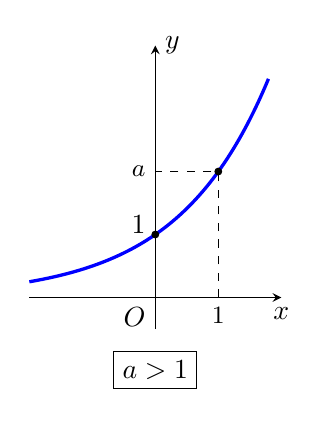
\begin{tikzpicture}[smooth,samples=300,scale=0.8,>=stealth]
			\draw[->] (-2,0)--(2,0) node[below]{$x$};
			\draw[->] (0,-0.5)--(0,4) node[right]{$y$};
			\draw (0,0) node[below left]{$O$};
			\draw[line width=1.2pt,color=blue,domain=-2:1.8] plot(\x,{2^(\x)});
			\draw[fill=black] (0,1) circle(1.5pt) (1,2) circle(1.5pt);
			\draw[dashed] (1,0)node[below]{\small $1$}--(1,2)--(0,2)node[left]{\small $a$};
			\node[below] at (0,-0.7) {\fbox{$a>1$}};
			\node[left] at (0,1.15) {$1$};
		\end{tikzpicture}
		\hspace{2cm}
		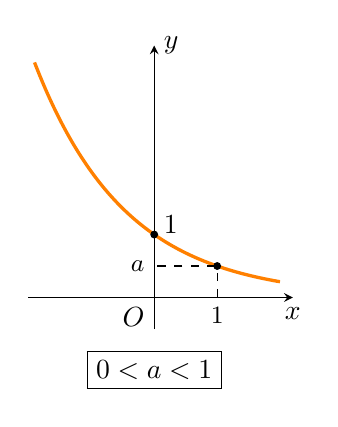
\begin{tikzpicture}[smooth,samples=300,scale=0.8,>=stealth]
			\draw[->] (-2,0)--(2.2,0) node[below]{$x$};
			\draw[->] (0,-0.5)--(0,4) node[right]{$y$};
			\draw (0,0) node[below left]{$O$};
			\draw[line width=1.2pt,color=orange,domain=-1.9:2] plot(\x,{0.5^(\x)});
			\draw[fill=black] (0,1) circle(1.5pt) (1,0.5) circle(1.5pt);
			\draw[dashed] (1,0)node[below]{\small $1$}--(1,0.5)--(0,0.5)node[left]{\small $a$};
			\node[below] at (0,-0.7) {\fbox{$0<a<1$}};
			\node[right] at (0,1.15) {$1$};
		\end{tikzpicture}
	\end{center}
\end{khung4}

\subsubsection{Hàm số logarit}
\indam{Định nghĩa:}
\begin{boxdn}
	Cho số thực $a>0$ và khác $1$. Hàm số $y=\log_a x$ được gọi là hàm số logarit cơ số $a$.
\end{boxdn}
\begin{khung4}{Tính chất}
	Hàm số logarit $y=\log_ax$, trong đó $0<a \ne 1$:
	\begin{itemize}
		\item Có tập xác định là $(0;+\infty)$ và tập giá trị là $\mathbb{R}$;
		\item Đồng biến trên $(0 ;+\infty)$ khi $a>1$ và nghịch biến trên $(0 ;+\infty)$ khi $0<a<1$; 
		\item Liên tục trên $(0 ;+\infty)$;
		\item Có đồ thị đi qua các điểm $(1 ; 0),(a ; 1)$ và luôn nằm bên phải trục tung.
	\end{itemize}
	\begin{center}
		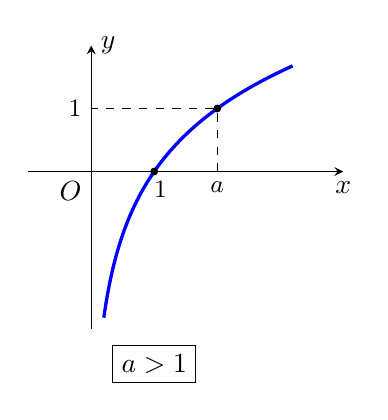
\begin{tikzpicture}[smooth,samples=300,scale=0.8,>=stealth]
			\draw[->] (-1,0)--(4,0) node[below]{$x$};
			\draw[->] (0,-2.5)--(0,2) node[right]{$y$};
			\draw (0,0) node[below left]{$O$};
			\draw[line width=1.2pt,color=blue,domain=0.2:3.2]plot(\x,{ln((\x))/ln(2)});
			\draw[fill=black] (1,0) circle(1.5pt) (2,1) circle(1.5pt);
			\draw[dashed] (2,0)node[below]{\small $a$}--(2,1)--(0,1)node[left]{\small $1$};
			\node[below] at (1,-2.6) {\fbox{$a>1$}};
			\node[below] at (1.1,0) {\small $1$};\end{tikzpicture}
		\hspace{2cm}
		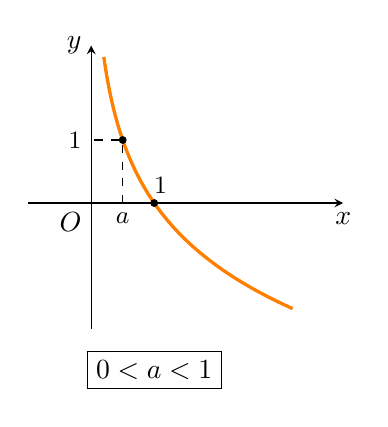
\begin{tikzpicture}[smooth,samples=300,scale=0.8,>=stealth]
			\draw[->] (-1,0)--(4,0) node[below]{$x$};
			\draw[->] (0,-2)--(0,2.5) node[left]{$y$};
			\draw (0,0) node[below left]{$O$};
			\draw[line width=1.2pt,color=orange,domain=0.2:3.2]plot(\x,{ln((\x))/ln(0.5)});
			\draw[fill=black] (1,0) circle(1.5pt) (0.5,1) circle(1.5pt);
			\draw[dashed] (0.5,0)node[below]{\small $a$}--(0.5,1)--(0,1)node[left]{\small $1$};
			\node[below] at (1,-2.2) {\fbox{$0<a<1$}};
			\node[above] at (1.1,0) {\small $1$};
		\end{tikzpicture}
	\end{center}
\end{khung4}
\subsubsection{Liên hệ đồ thị của hai hàm số}
\immini{
	Đồ thị hàm số $y=a^x$ và $y=\log_ax$ đối xứng nhau qua đường phân giác của góc phần tư (đường thẳng $y=x$) thứ nhất.
}{
	\hspace{1cm}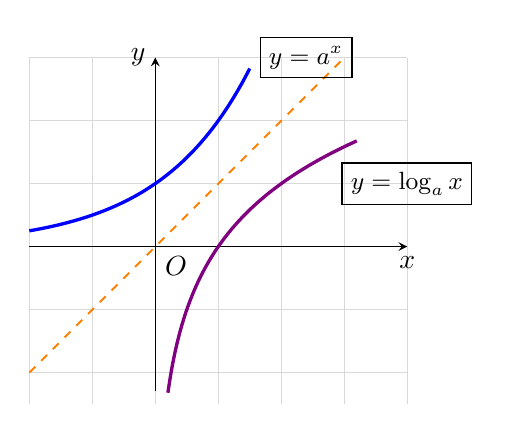
\begin{tikzpicture}[smooth,samples=300,scale=0.8,>=stealth]
		\draw [color=gray!30,, xstep=1.0cm,ystep=1.0cm] (-2,-2.5) grid (4,3);
		\draw[->] (-2,0)--(4,0) node[below]{$x$};
		\draw[->] (0,-2.3)--(0,3) node[left]{$y$};
		\draw (0,0) node[below right]{$O$};
		\draw[line width=1.2pt,color=blue,domain=-2:1.5] plot(\x,{2^(\x)});
		\draw[line width=1.2pt,color=violet,domain=0.2:3.2]plot(\x,{ln((\x))/ln(2)});
		\draw[dashed,line width=0.7pt,color=orange] (-2,-2)--(3,3);
		%\node[below] at (2,-1.2) {\small\fbox{Hình I.3}};
		\node[right] at (2.8,1) {\small\fbox{$y=\log_ax$}};
		\node[right] at (1.5,3) {\small\fbox{$y=a^x$}};
	\end{tikzpicture}
}

%%Phần 2: Phân dạng 

\subsection{PHÂN LOẠI VÀ PHƯƠNG PHÁP GIẢI TOÁN}
\begin{dang}{Xác định hàm số mũ, hàm số logarit}
	Cho số thực $a>0$ và khác $1$. Khi đó:
	\begin{listEX}[1]
		\item [\ding{172}] Hàm số $y=a^x$ được gọi là hàm số mũ cơ số $a$.
		\item [\ding{172}] Hàm số $y=\log_a x$ được gọi là hàm số logarit cơ số $a$.
	\end{listEX}
\end{dang}
\indam{Ví dụ minh hoạ}
\begin{vd}%[1D6N3-1]%[Dự án đề cương 3 khối NH 24-25-Dot 1- Nắng Đông]
	Trong các hàm số sau đây, hàm số nào là hàm số mũ? Chỉ ra cơ số của nó.
	\begin{multicols}{3}
		\begin{enumerate}
			\item $y=3^{\tfrac{x}{2}}$;
			\item $y=x^{-4}$;
			\item $y=4^{-x}$.
		\end{enumerate}	
	\end{multicols}
	\loigiai{\begin{enumerate}
			\item $y=3^{\tfrac{x}{2}}=\left(3^{\tfrac{1}{2}}\right)^x=\left(\sqrt{3}\right)^x$ là hàm số mũ với cơ số $a=\sqrt{3}$.
			\item $y=x^{-4}$ không phải là hàm số mũ.
			\item $y=4^{-x}=\left(4^{-1}\right)^x=\left(\dfrac{1}{4}\right)^x$ là hàm số mũ với cơ số $a=\dfrac{1}{4}$.
	\end{enumerate}}
\end{vd}

\begin{vd}%[1D6N3-1]%[Dự án đề cương 3 khối NH 24-25-Dot 1- Nắng Đông]
	Trong các hàm số sau, hàm số nào là hàm số logarit? Chỉ ra cơ số của nó.
	\begin{multicols}{3}
		\begin{enumerate}
			\item $y=\log_{\sqrt{2}}x$;
			\item $y=-\log_3x$;
			\item $y=x\log_23$.
		\end{enumerate}	
	\end{multicols}
	\loigiai{\begin{enumerate}
			\item $y=\log_{\sqrt{2}}x$ là hàm số logarit với cơ số $a=\sqrt{2}$.
			\item $y=-\log_3x=\log_{\tfrac{1}{3}}x$ là hàm số logarit với cơ số $a=\dfrac{1}{3}$.
			\item $y=x\log_23$ không phải là hàm số logarit (mà là hàm số bậc nhất với hệ số góc bằng $\log_23$).
	\end{enumerate}}
\end{vd}

\begin{dang}{Tìm tập xác định của hàm số mũ và hàm số logarit}
	Cho số thực $a>0$ và khác $1$. Khi đó:
	\begin{listEX}[1]
		\item [\ding{172}] Hàm số $y=a^x$ xác định với mọi $x\in \mathbb{R}$.
		\item [\ding{172}] Hàm số $y=\log_a x$ xác định với mọi $x>0$.
		\item [\ding{172}] Hàm số $y=a^{f(x)}$ xác định khi và chi khi $f(x)$ có nghĩa.
		\item [\ding{172}] Hàm số $y=\log_a {f(x)}$ xác định khi và chỉ khi $f(x)>0$.
	\end{listEX}
\end{dang}
\indam{Ví dụ minh hoạ}
\begin{vd}%[1D6H3-2]%[Dự án đề cương 3 khối NH 24-25-Dot 1- Nắng Đông]
	Tìm tập xác định của mỗi hàm số sau
	\begin{multicols}{3}
		\begin{enumerate}
			\item $y=5^{x^4+3x-2}$;
			\item $y=7^{\tfrac{x^2-2x+2}{3-x}}$;
			\item $y=2^{\sqrt{x+3}}$.
		\end{enumerate}	
	\end{multicols}
	\loigiai{
		\begin{enumerate}
			\item Điều kiện xác định: $x\in \mathbb{R}$.\\
			Vậy tập xác định của hàm số đã cho là $\mathscr{D}=\mathbb{R}$.
			\item Điều kiện xác định: $3-x \neq 0 \Leftrightarrow x\neq 3$.\\
			Vậy tập xác định của hàm số đã cho là $\mathscr{D}=\mathbb{R}\setminus\left\{3\right\}$.
			\item Điều kiện xác định: $x+3\geq 0\Leftrightarrow x\geq -3$.\\
			Vậy tập xác định của hàm số đã cho là $\mathscr{D}=[-3;+\infty)$.
		\end{enumerate}	
	}
\end{vd}

\begin{vd}%[1D6H3-2]%[Dự án đề cương 3 khối NH 24-25-Dot 1- Nắng Đông]
	Tìm tập xác định của mỗi hàm số sau
	\begin{multicols}{3}
		\begin{enumerate}
			\item $y=\log_3\left(5x-3\right)$;
			\item $y=\log_6\left(5-4x-x^2\right)$.
		\end{enumerate}	
	\end{multicols}
	\loigiai{
		\begin{enumerate}
			\item Điều kiện xác định: $5x-3>0\Leftrightarrow x>\dfrac{3}{5}$.\\
			Vậy tập xác định của hàm số đã cho là $\mathscr{D}=\left(\dfrac{3}{5};+\infty\right)$.
			\item Điều kiện xác định: $5-4x-x^2>0\Rightarrow -5<x<1$.\\
			Vậy tập xác định của hàm số đã cho là $\mathscr{D}=\left(-5;1\right)$.
		\end{enumerate}	
	}
\end{vd}

\begin{vd}%[1D6V3-2]%[Dự án đề cương 3 khối NH 24-25-Dot 1- Nắng Đông]
	Tìm tất cả giá trị của tham số $m$ để hàm số $y=\log \left (x^2-2mx+4 \right )$ xác định với mọi $x$ thuộc $\mathbb{R}$.
	\loigiai
	{Điều kiện xác định: $x^2-2mx+4>0$.\\
	Hàm số đã cho xác định với mọi $x\in\mathbb{R}$ thì $x^2-2mx+4>0,\,\,\forall x\in\mathbb{R}$
		$$\Leftrightarrow \heva{& a=1>0\\&\Delta'=m^2-4<0}\Leftrightarrow -2<m<2.$$
	Vậy $-2<m<2$ là giá trị cần tìm.
	}
\end{vd}
\begin{dang}{Vẽ đồ thị hàm số mũ, hàm số logarit}
Các bước khảo sát và vẽ đồ thị hàm số mũ $y=a^x$, với $0<a \ne 1$.
	\begin{itemize}
		\item Tìm tập xác định là $\mathscr{D}=\mathbb{R}$;
		\item Nhận xét tính đơn điệu của hàm số: đồng biến trên $\mathbb{R}$ khi $a>1$ và nghịch biến trên $\mathbb{R}$ khi $0<a<1$.
		\item Lập bảng biến thiên;
		\item Lập bảng giá trị: đồ thị đi qua các điểm $(0;1),(1;a)$.
		\item Vẽ đồ thị.
	\end{itemize}
	\begin{center}
		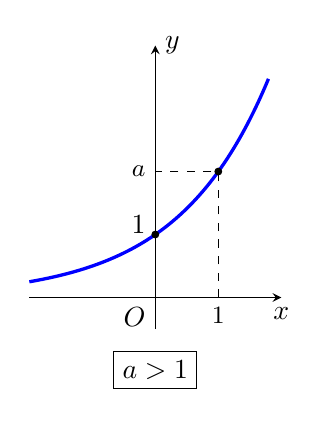
\begin{tikzpicture}[smooth,samples=300,scale=0.8,>=stealth]
			\draw[->] (-2,0)--(2,0) node[below]{$x$};
			\draw[->] (0,-0.5)--(0,4) node[right]{$y$};
			\draw (0,0) node[below left]{$O$};
			\draw[line width=1.2pt,color=blue,domain=-2:1.8] plot(\x,{2^(\x)});
			\draw[fill=black] (0,1) circle(1.5pt) (1,2) circle(1.5pt);
			\draw[dashed] (1,0)node[below]{\small $1$}--(1,2)--(0,2)node[left]{\small $a$};
			\node[below] at (0,-0.7) {\fbox{$a>1$}};
			\node[left] at (0,1.15) {$1$};
		\end{tikzpicture}
		\hspace{2cm}
		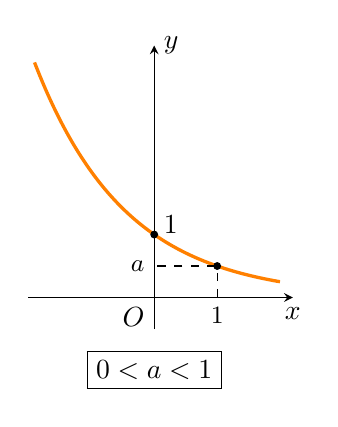
\begin{tikzpicture}[smooth,samples=300,scale=0.8,>=stealth]
			\draw[->] (-2,0)--(2.2,0) node[below]{$x$};
			\draw[->] (0,-0.5)--(0,4) node[right]{$y$};
			\draw (0,0) node[below left]{$O$};
			\draw[line width=1.2pt,color=orange,domain=-1.9:2] plot(\x,{0.5^(\x)});
			\draw[fill=black] (0,1) circle(1.5pt) (1,0.5) circle(1.5pt);
			\draw[dashed] (1,0)node[below]{\small $1$}--(1,0.5)--(0,0.5)node[left]{\small $a$};
			\node[below] at (0,-0.7) {\fbox{$0<a<1$}};
			\node[right] at (0,1.15) {$1$};
		\end{tikzpicture}
	\end{center}
	
Các bước khảo sát và vẽ đồ thị của hàm số logarit $y=\log_ax$, với $0<a \ne 1$.
	\begin{itemize}
		\item Tìm tập xác định là $\mathscr{D}=(0;+\infty)$;
		\item Nhận xét tính đơn điệu của hàm số: đồng biến trên $(0 ;+\infty)$ khi $a>1$ và nghịch biến trên $(0 ;+\infty)$ khi $0<a<1$; 
		\item Lập bảng biến thiên;
		\item Lập bảng giá trị: đồ thị đi qua các điểm $(1;0)$, $(a;1)$;
		\item Vẽ đồ thị.
	\end{itemize}
	\begin{center}
		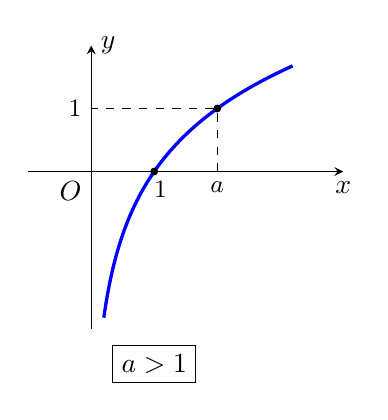
\begin{tikzpicture}[smooth,samples=300,scale=0.8,>=stealth]
			\draw[->] (-1,0)--(4,0) node[below]{$x$};
			\draw[->] (0,-2.5)--(0,2) node[right]{$y$};
			\draw (0,0) node[below left]{$O$};
			\draw[line width=1.2pt,color=blue,domain=0.2:3.2]plot(\x,{ln((\x))/ln(2)});
			\draw[fill=black] (1,0) circle(1.5pt) (2,1) circle(1.5pt);
			\draw[dashed] (2,0)node[below]{\small $a$}--(2,1)--(0,1)node[left]{\small $1$};
			\node[below] at (1,-2.6) {\fbox{$a>1$}};
			\node[below] at (1.1,0) {\small $1$};\end{tikzpicture}
		\hspace{2cm}
		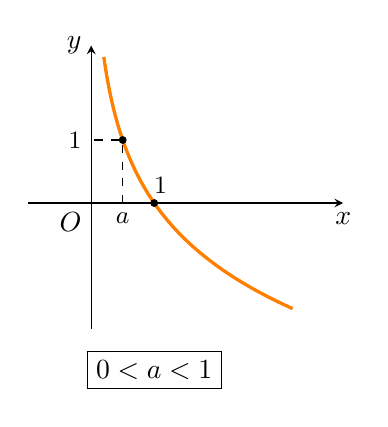
\begin{tikzpicture}[smooth,samples=300,scale=0.8,>=stealth]
			\draw[->] (-1,0)--(4,0) node[below]{$x$};
			\draw[->] (0,-2)--(0,2.5) node[left]{$y$};
			\draw (0,0) node[below left]{$O$};
			\draw[line width=1.2pt,color=orange,domain=0.2:3.2]plot(\x,{ln((\x))/ln(0.5)});
			\draw[fill=black] (1,0) circle(1.5pt) (0.5,1) circle(1.5pt);
			\draw[dashed] (0.5,0)node[below]{\small $a$}--(0.5,1)--(0,1)node[left]{\small $1$};
			\node[below] at (1,-2.2) {\fbox{$0<a<1$}};
			\node[above] at (1.1,0) {\small $1$};
		\end{tikzpicture}
	\end{center}
	
\end{dang}
\indam{Ví dụ minh hoạ}
\begin{vd}%[1D6H3-3]%[Dự án đề cương 3 khối NH 24-25-Dot 1- Nắng Đông]
	Lập bảng biến thiên và vẽ đồ thị hàm số $y=3^x$.
	\loigiai{
		\immini{
			Tập xác định $\mathscr{D}=\mathbb{R}$.\\
			Vì hàm số $y=3^x$ có cơ số $3>1$ nên hàm số $y=3^x$ đồng biến trên $\mathbb{R}$, ta có bảng biến thiên như sau
			\begin{center}
				
\begin{tikzpicture}[>=stealth,line join=round,line cap=round,font=\footnotesize]
					\tkzTabInit[nocadre=false,lgt=2,espcl=2,deltacl=0.5]{$x$/0.7,$y=3^x$/2}
					{$-\infty$ , $0$ , $+\infty$}
					\tkzTabVar{-/$0$ , R , +/$+\infty$}
					\tkzTabIma{1}{3}{2}{$1$}% Từ cột 1 đến cột 3 đặt f(2) tại cột 2.
				\end{tikzpicture}
			\end{center}
			Bảng giá trị
			\begin{center}
				\begin{tabular}{|c|c|c|c|c|}
					\hline
					$x$  & $-1$ & $0$ & $1$ & $2$ \\
					\hline
					$y=3^{x}$& $\dfrac{1}{3}$ & $1$ & $3$ & $9$ \\
					\hline
				\end{tabular}
			\end{center}
			Đồ thị của hàm số $y=3^x$ là một đường cong liền nét đi qua các điểm $A\left(-1;\dfrac{1}{3}\right)$, $B(0;1)$, $C(1;3)$, $D(2;9)$.
		}{
			\begin{tikzpicture}[>=stealth,line join=round,line cap=round,font=\footnotesize,scale=0.55]
				\def\a{3}
				\draw[->] (-4,0) -- (5,0) node[below] {$x$};
				\draw[->] (0,-2) -- (0,10) node[left] {$y$};
				\draw (0,0)node[below right=-0.1]{$O$};
				\clip (-4,-5)rectangle(5,10);
				\draw[line width=1.2pt,color=red,samples=200,smooth,domain=-3:4] plot(\x, {\a^\x});
				\draw[dashed] (0,3)--(1,3) node[right]{$C$}--(1,0);
				\draw[dashed] (0,9)--(2,9)node[right]{$D$}--(2,0);
				\draw[dashed] (-1,0)--(-1,1/3)node[above left]{$A$}--(0,1/3)node[right]{$\frac{1}{3}$};
				\draw (0,1) node [above left=-0.1] {$1$}node[right]{$B$};
				\draw (1,0) node [below] {$1$};
				\draw (0,3) node [left] {$3$};
				\draw (2,0) node [below] {$2$};
				\draw (0,9) node [left] {$9$};
				\draw (-1,0) node [below] {$-1$};
			\end{tikzpicture}
		}
	}
\end{vd}
\begin{vd}%[1D6H3-3]%[Dự án đề cương 3 khối NH 24-25-Dot 1- Nắng Đông]
	Lập bảng biến thiên và vẽ đồ thị hàm số $y=\left(\dfrac{1}{2}\right)^{x}$.
	\loigiai{
		\immini{
			Tập xác định $\mathscr{D}=\mathbb{R}$.\\
			Vì hàm số $y=\left(\dfrac{1}{2}\right)^{x}$ có cơ số $\dfrac{1}{2}<1$ nên hàm số $y=\left(\dfrac{1}{2}\right)^{x}$ nghịch biến trên $\mathbb{R}$, ta có bảng biến thiên như sau
			\begin{center}
				
\begin{tikzpicture}[>=stealth,line join=round,line cap=round,font=\footnotesize]
					\tkzTabInit[nocadre=false,lgt=2,espcl=2,deltacl=0.5]{$x$/0.7,$y=\left(\dfrac{1}{2}\right)^{x}$/2}
					{$-\infty$ , $0$ , $+\infty$}
					\tkzTabVar{+/$0$ , R , -/$+\infty$}
					\tkzTabIma{1}{3}{2}{$1$}% Từ cột 1 đến cột 3 đặt f(2) tại cột 2.
				\end{tikzpicture}
			\end{center}
		Bảng giá trị
		\begin{center}
			\begin{tabular}{|c|c|c|c|c|c|}
				\hline
				$ x $  & $-2$ & $-1$ & $0$ & $1$ \\
				\hline
				$y = \left(\dfrac{1}{2}\right)^{x}$& $4$ & $2$ & $1$ & $\dfrac{1}{2}$ \\
				\hline
			\end{tabular}
		\end{center}
			Đồ thị của hàm số $y=\left(\dfrac{1}{2}\right)^{x}$ là một đường cong liền nét đi qua các điểm $A\left(1;\dfrac{1}{2}\right)$, $B(0;1)$, $C(-1;2)$, $D(-2;4)$.
		}{
			\begin{tikzpicture}[>=stealth,line join=round,line cap=round,font=\footnotesize,scale=0.9]
				\draw[->] (-3,0)--(3,0) node[below]{$x$};
				\draw[->] (0,-1)--(0,5) node[right]{$y$};
				\draw (0,0) node[below left]{$O$};
				\draw[line width=1.2pt,color=red,domain=-2.2:2.8] plot(\x,{0.5^(\x)});
				\draw[fill=black] (0,1) circle(1pt)node[left]{$B$} (0,2) circle(1pt) (0,3) circle(1pt) (0,4) circle(1pt)  (-2,0) circle(1pt) (-1,0) circle(1pt) (1,0) circle(1pt) (4,0) circle(1pt);
				\draw[dashed] (-2,0)node[below]{\small $-2$}--(-2,4)node[left]{$D$}--(0,4)node[right]{\small $4$};
				\draw[dashed] (-1,0)node[below]{\small $-1$}--(-1,2)node[left]{$C$}--(0,2)node[right]{\small $2$};
				\draw[dashed] (0,1/2)node[left]{\small $\frac{1}{2}$}--(1,1/2)node[above right]{$A$}--(1,0)node[below]{\small $1$};
				\node[right] at (0,1.15) {$1$};
			\end{tikzpicture}
		}	
	}
\end{vd}

\begin{vd}%[1D6H3-3]%[Dự án đề cương 3 khối NH 24-25-Dot 1- Nắng Đông]
	Lập bảng biến thiên và vẽ đồ thị hàm số $y=\log_3 x$.
	\loigiai{
		\immini{
			Tập xác định $\mathscr{D}=(0;+\infty)$.\\
			Vì hàm số $y=\log_3 x$ có cơ số $3>1$ nên hàm số $y=\log_3 x$ đồng biến trên khoảng $(0;+\infty)$, ta có bảng biến thiên như sau
			\begin{center}
				
\begin{tikzpicture}[>=stealth,line join=round,line cap=round,font=\footnotesize]
					\tkzTabInit[nocadre=false,lgt=2.3,espcl=2,deltacl=0.5]{$x$/0.7,$y=\log_3x$/2}
					{$0$ , $1$ , $+\infty$}
					\tkzTabVar{-/$-\infty$ , R , +/$+\infty$}
					\tkzTabIma{1}{3}{2}{$0$}% Từ cột 1 đến cột 3 đặt f(2) tại cột 2.
				\end{tikzpicture}
			\end{center}
			Bảng giá trị
			\begin{center}
				\begin{tabular}{|c|c|c|c|c|}
					\hline
					$x$  & $\dfrac{1}{3}$ & $1$ & $3$ & $9$ \\
					\hline
					$y=\log_3 x$& $-1$ & $0$ & $1$ & $2$ \\
					\hline
				\end{tabular}
			\end{center}
			Đồ thị của hàm số $y=\log_3 x$ là một đường cong liền nét đi qua các điểm $A\left(\dfrac{1}{3};-1\right)$, $B(1;0)$, $C(3;1)$, $D(9;2)$.
		}{
			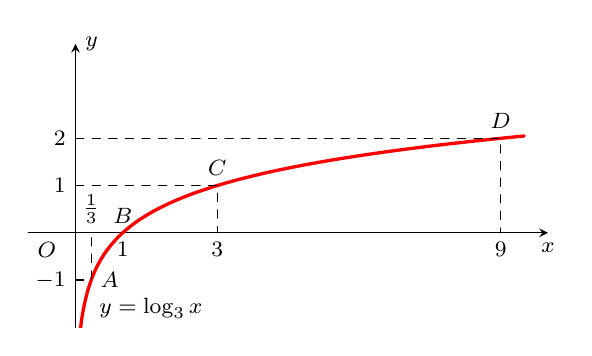
\begin{tikzpicture}[>=stealth,line join=round,line cap=round,font=\footnotesize,scale=0.6]
				\draw[->](-1,0) -- (10,0) node[below]{ $x$};
				\draw[->](0,-2) -- (0,4) node[below,right]{ $y$};
				\draw(-0.2,0) node[below left]{\footnotesize $O$};
				\clip(-1,-2) rectangle (10,4);
				\draw[line width=1.2pt,color=red,smooth,samples=300,domain=0.1:9.5]plot(\x,{ln(\x)/ln(3)});
				\draw(1,0) node[below]{$1$}node[above]{$B$};
				\draw[dashed] (0,1) node[left]{$1$}--(3,1)node[above]{$C$}--(3,0)node[below]{$3$};
				\draw[dashed] (0,2) node[left]{$2$}--(9,2)node[above]{$D$}--(9,0)node[below]{$9$};
				\draw[dashed] (0,-1) node[left]{$-1$}--(1/3,-1)node[right]{$A$}--(1/3,0)node[above]{$\frac{1}{3}$};
				\draw (0.3,-1.6)node[right]{$y=\log_3x$};
			\end{tikzpicture}
		}
	}
\end{vd}

\begin{dang}{Các bài toán liên quan đồ thị của hàm số mũ, hàm số logarit}
	Cho $a$, $b$ là hai số thực dương khác $1$. Khi đó
	\begin{itemize}
		\item [\ding{172}] Với $m>0$ và $a^m>b^m$ thì $a>b$;
		\item [\ding{172}] Với $m<0$ và $a^m>b^m$ thì $a<b$;
	\end{itemize}
\end{dang}
\indam{Ví dụ minh hoạ}
\begin{vd}%[1D6H3-3]%[Dự án đề cương 3 khối NH 24-25-Dot 1- Nắng Đông]
	\immini{
		Đường cong trong hình sau là đồ thị của hàm số $y=\left(\sqrt{a}\right)^x$, với $a$ là số thực dương khác $1$. Tính giá trị của biểu thức $T=25a-26$.
	}{
		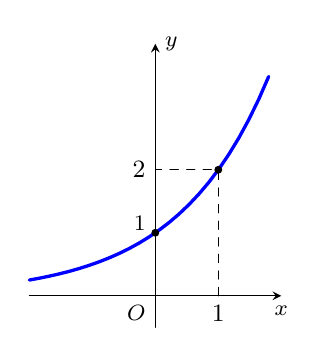
\begin{tikzpicture}[>=stealth,line join=round,line cap=round,font=\footnotesize,scale=0.8]
			\draw[->] (-2,0)--(2,0) node[below]{$x$};
			\draw[->] (0,-0.5)--(0,4) node[right]{$y$};
			\draw (0,0) node[below left]{$O$};
			\draw[line width=1.2pt,color=blue,domain=-2:1.8] plot(\x,{2^(\x)});
			\draw[fill=black] (0,1) circle(1.5pt) (1,2) circle(1.5pt);
			\draw[dashed] (1,0)node[below]{\small $1$}--(1,2)--(0,2)node[left]{\small $2$};
			\node[left] at (0,1.15) {$1$};
		\end{tikzpicture}
	}
	\loigiai{
		Đồ thị của hàm số $y=\left(\sqrt{a}\right)^x$ đi qua điểm có tọa độ $A(1;2)$ nên $$2=\sqrt{a}\Leftrightarrow a=4.$$
		Vậy $T=25a-26=25\cdot 4-16=84.$
	}
\end{vd}

\begin{vd}%[1D6H3-3]%[Dự án đề cương 3 khối NH 24-25-Dot 1- Nắng Đông]
	\immini{Trên hình vẽ, đồ thị của ba hàm số $y=a^x$, $y=b^x$, $y=c^x$ ($a$, $b$, $c$ là ba số dương khác $1$ cho trước) được vẽ trong cùng một mặt phẳng tọa độ. Dựa vào đồ thị và các tính chất của lũy thừa, hãy so sánh ba số $a$, $b$ và $c$.}
	{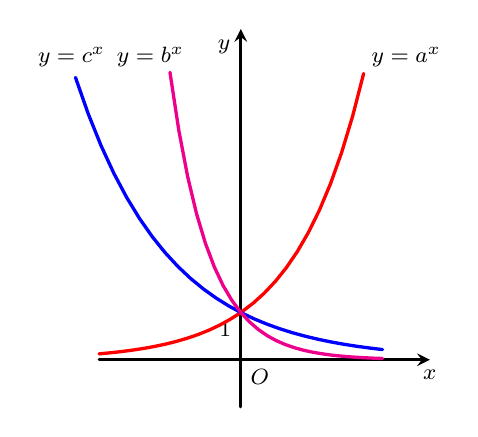
\begin{tikzpicture}[>=stealth,line join=round,line cap=round,font=\footnotesize,scale=0.6]
			\draw[->,line width = 1pt] (-3,0)--(4,0) node[below]{$x$};
			\draw(0,0)node[below right]{$O$} circle (1pt);
			\draw(0,1)node[below left]{$1$} circle (1pt);
			\draw[->,line width = 1pt] (0,-1) --(0,7) node[below left]{$y$};
			\draw [line width=1.2pt,color=red, domain=-3:2.6] plot (\x, {2^\x});
			\draw (3.5,6) node[above]{$y=a^x$};
			\draw [line width=1.2pt,color=blue, domain=-3.5:3] plot (\x, {(0.6)^\x});
			\draw (-4.5,6) node[above right]{$y=c^x$};
			\draw [line width=1.2pt,color=magenta, domain=-1.5:3] plot (\x, {(0.3)^\x});
			\draw (-1,6) node[above left]{$y=b^x$};
	\end{tikzpicture}}
	\loigiai{Từ đồ thị ta thấy
		\begin{itemize}
			\item Hàm số $y=a^x$ đồng biến trên $\mathbb{R}$ nên $a>1$.
			\item Hàm số $y=c^x$, $y=b^x$ nghịch biến trên $\mathbb{R}$, do đó $0<b,c<1$.
		\end{itemize}
		Lại có $x>0\Rightarrow c^x>b^x$ và $x<0\Rightarrow c^x<b^x$ nên $c>b$.\\
		Vậy $a>c>b$.}
\end{vd}

\begin{dang}{Các bài toán liên quan tính đơn điệu của hàm số mũ, hàm số logarit}
	Cho $a$ là số thực dương khác $1$ và hai số thực $m$, $n$. Khi đó:
	\begin{listEX}[1]
		\item [\ding{172}] $a>1$ thì $a^m>a^n\Leftrightarrow m>n$;
		\item [\ding{172}] $0<a<1$ thì $a^m>a^n\Leftrightarrow m<n$;
		\item [\ding{172}] $a>1$ thì $\log_a m>\log_a n \Leftrightarrow m>n$, với $m>0$ và $n>0$;
		\item [\ding{172}] $0<a<1$ thì $\log_a m>\log_a n \Leftrightarrow m<n$, với $m>0$ và $n>0$.
	\end{listEX}
\end{dang}
\indam{Ví dụ minh hoạ}
\begin{vd}%[1D6H3-3]%[Dự án đề cương 3 khối NH 24-25-Dot 1- Nắng Đông]
	Sử dụng tính chất của hàm số mũ, so sánh các cặp số sau
	\begin{multicols}{3}
		\begin{enumerate}
			\item $\pi^2$ và $\pi^{\sqrt{3}}$;
			\item $\left(\dfrac{6}{7}\right)^{-3}$ và $\left(\dfrac{6}{7}\right)^{-5}$;
			\item $\sqrt[5]{16}$ và $\sqrt[7]{64}$.
		\end{enumerate}
	\end{multicols}
	\loigiai{\begin{enumerate}
			\item Ta có $\pi>1$ nên hàm số $y=\pi^x$ đồng biến trên $\mathbb{R}$.\\ Mà $2>\sqrt{3}$ nên $\pi^2>\pi^{\sqrt{3}}$.
			\item Ta có $\dfrac{6}{7}<1$ nên hàm số $y=\left(\dfrac{6}{7}\right)^x$ nghịch biến trên $\mathbb{R}$.\\ Mà $-3>-5$ nên $\left(\dfrac{6}{7}\right)^{-3}<\left(\dfrac{6}{7}\right)^{-5}$.
			\item Ta có $\sqrt[5]{16}=\sqrt[5]{2^4}=2^{\tfrac{4}{5}}$ và $\sqrt[7]{64}=\sqrt[7]{2^6}=2^{\tfrac{6}{7}}$.
			Vì $2>1$ nên hàm số $y=2^x$ đồng biến trên $\mathbb{R}$.\\ Mà $\dfrac{4}{5}<\dfrac{6}{7}$ nên $2^{\tfrac{4}{5}}<2^{\tfrac{6}{7}}$, suy ra $\sqrt[5]{16}<\sqrt[7]{64}$.
	\end{enumerate}}
\end{vd}

\begin{vd}%[1D6H3-4]%[Dự án đề cương 3 khối NH 24-25-Dot 1- Nắng Đông]
	Sử dụng tính chất của hàm số logarit, so sánh các cặp số sau
	\begin{multicols}{2}
		\begin{enumerate}
			\item $\log_280$ và $4\log_23$;
			\item $2\log_{0{,}7}7$ và $3\log_{0{,}7}4$.
		\end{enumerate}
	\end{multicols}
	\loigiai{\begin{enumerate}
			\item Ta có $4\log_23=\log_23^4=\log_281$.\\
			Hàm số $y=\log_3x$ có cơ số $3>1$ nên đồng biến trên khoảng $(0;+\infty)$.\\
			Mà $80<81$ nên $\log_280<\log_281$.\\ Vậy $\log_280<4\log_23$.
			\item Ta có $2\log_{0{,}7}7=\log_{0{,}7}7^2=\log_{0{,}7}49$ và $3\log_{0{,}7}4=\log_{0{,}7}4^3=\log_{0{,}7}64$.\\
			Hàm số $y=\log_{0{,}7}x$ có cơ số $0{,}7<1$ nên nghịch biến trên khoảng $(0;+\infty)$.\\
			Mà $49<64$ nên $\log_{0{,}7}49>\log_{0{,}7}64$.\\ Vậy $2\log_{0{,}7}7>3\log_{0{,}7}4$.
	\end{enumerate}}
\end{vd}
\begin{dang}{Các bài toán ứng dụng hàm số mũ, hàm số logarit vào thực tiễn}
	\indam{Bài toán lãi kép}\\
	\textbf{- Bài toán 1.} Ông A gửi số tiền $P$ đồng vào ngân hàng T với lãi suất $r$ một năm ($r$ tính theo $\%$). Biết rằng nếu không rút tiền ra khỏi ngân hàng thì cứ sau mỗi năm, số tiền lãi sẽ được nhập vào vốn ban đầu. Hỏi ông A được lãnh bao nhiêu tiền (cả vốn ban đầu và lãi) sau $n$ năm, nếu trong khoảng thời gian này không rút tiền ra và lãi suất không thay đổi?\\
		Số tiền ông A được lãnh sau $n$ năm là 
		\begin{center}
			$P_n=P(1+r)^n$. 
		\end{center}
	\textbf{- Bài toán 2.} Đầu mỗi tháng, bà B gửi số tiền $P$ đồng vào ngân hàng N với lãi suất $r$ một tháng ($r$ tính theo $\%$). Hỏi bà B được lãnh bao nhiêu tiền (cả vốn ban đầu và lãi) sau $n$ tháng, nếu trong khoảng thời gian này không rút tiền ra và lãi suất không thay đổi?\\ 
		Số tiền bà B được lãnh sau $n$ tháng là 
		\begin{center}
			$S_n=\dfrac{P}{r}\left[ (1+r)^n-1\right]\cdot(1+r)$. 
		\end{center}
	\textbf{- Bài toán 3.} Anh C gửi số tiền $P$ đồng vào ngân hàng N với lãi suất $r$ một tháng ($r$ tính theo $\%$). Mỗi tháng anh C vào ngân hàng này tính lãi, rút ra số tiền $Q$ đồng. Hỏi số tiền còn lại sau $n$ tháng là bao nhiêu?\\
		Số tiền còn lại của anh C sau $n$ tháng là
		\begin{center}
			$S_n=P(1+r)^n-Q\dfrac{(1+r)^n-1}{r}$. 
		\end{center}
\end{dang}
\indam{Ví dụ minh hoạ}
\begin{vd}%%[1D6H3-5]%[Dự án đề cương 3 khối NH 24-25-Dot 1- Nắng Đông]
	Ông Nam gửi số tiền $30$ triệu đồng vào ngân hàng T với lãi suất $7\%$ một năm. Biết rằng nếu không rút tiền ra khỏi ngân hàng thì cứ sau mỗi năm, số tiền lãi sẽ được nhập vào vốn ban đầu. Hỏi ông Nam được lãnh bao nhiêu triệu đồng (cả vốn ban đầu và lãi) sau $4$ năm, nếu trong khoảng thời gian này không rút tiền ra và lãi suất không thay đổi? (kết quả làm tròn đến hàng phần chục).
	\loigiai{ Theo đề ta có $P=30$, $r=0{,}07$, $n=4$.\\
		Số tiền ông Nam được lãnh sau $4$ năm là $$P_4=30(1+0{,}07)^4 \approx 39{,}3 \text{ (triệu đồng) }.$$
	}
\end{vd}
%
\begin{vd}%[1D6H3-5]%[Dự án đề cương 3 khối NH 24-25-Dot 1- Nắng Đông]
	Đầu mỗi tháng, bà Nhung gửi số tiền $2$ triệu đồng vào ngân hàng N với lãi suất $0,5\%$ một tháng. Hỏi bà Nhung được lãnh bao nhiêu triệu đồng (cả vốn ban đầu và lãi) sau $3$ năm, nếu trong khoảng thời gian này không rút tiền ra và lãi suất không thay đổi? (kết quả làm tròn đến hàng phần chục).
	\loigiai{Theo đề ta có $P=2$, $r=0{,}005$, $n=36$.\\
		Số tiền bà Nhung được lãnh sau $3$ năm là $$S_{36}=\dfrac{2}{0{,}005}\left[ (1+0{,}005)^{36}-1\right]\cdot (1+0{,}005) \approx 79{,}1 \text{ (triệu đồng) }.$$
	}
\end{vd}

\begin{vd}%[1D6V3-5]%[Dự án đề cương 3 khối NH 24-25-Dot 1- Nắng Đông]
	Trong âm học, mức cường độ âm được tính bới công thức $L=10\log\left(\dfrac{I}{I_0}\right)$ (dB) (dB là đơn vị mức cường độ âm, đọc là đề-xi-ben), trong đó $I$ là cường độ âm tính theo W/m$^2$ và $I_0=10^{-12}$ W/m$^2$ là cường độ âm chuẩn (cường độ âm thấp nhất mà tai người bình thường có thể nghe được).
	\begin{center}
		(\textit{Nguồn:} Vật lí 12, NXB Giáo dục Việt Nam, năm 2017, trang 52,53)
	\end{center}
	\begin{enumerate}
		\item Mức cường độ âm $L$ thấp nhất mà tai người có thể nghe được là bao nhiêu?
		\item Cuộc trò chuyện có cường độ âm $10^{-9}$ W/m$^2$ thì có mức cường độ âm bằng bao nhiêu?
		\item Cường độ âm tại một khu văn phòng nằm trong miền từ $10^{-7}$ W/m$^2$ đến $5\cdot10^{-6}$ W/m$^2$ (tức là $10^{-7}\le I\le5\cdot10^{-6}$). Mức cường độ âm tại khu văn phòng này nằm trong khoảng nào? (Làm tròn kết quả đến hàng đơn vị).
	\end{enumerate}
	\loigiai{\begin{enumerate}
			\item Khi $I=I_0$ thì $L=10\log 1=0$ (dB).\\ Vậy mức cường độ âm thấp nhất mà tai người bình thường có thể nghe được là $0$ (dB).
			\item Khi $I=10^{-9}$ W/m$^2$, ta có $L=10\log\dfrac{10^{-9}}{10^{-12}}=10\log10^3=30\log10=30$ (dB).
			\item Với $I=10^{-7}$ W/m$^2$, $L=10\log\dfrac{10^{-7}}{10^{-12}}=10\log10^5=50\log10=50$ (dB).\\
			Với $I=5\cdot10^{-6}$ W/m$^2$, $L=10\log\dfrac{5\cdot10^{-6}}{10^{-12}}=10\log\left(5\cdot10^6\right)=10(6+\log5)\approx67$ (dB).\\
			Hàm số $y=\log x$ đồng biến nên hàm số $y=10\log x$ cũng đồng biến.\\
			Do đó, từ $10^{-7}\le I\le5\cdot10^{-6}$ suy ra $50\le L\le67$.\\
			Vậy mức cường độ âm tại khu văn phòng nằm trong khoảng từ $50$ (dB) đến $67$ (dB).
	\end{enumerate}}
\end{vd}
%-----------------------------------------------------------------------------
\subsection{Bài tập rèn luyện}
\ind{PHẦN I.} \inden{Câu trắc nghiệm nhiều phương án lựa chọn. Mỗi câu hỏi học sinh chỉ chọn một phương án.}\\
\setcounter{ex}{0}
\Opensolutionfile{ans}[ans/2D1-Bai1-TN]%--Đặt tên 2D1-Bai1-Dang1-TN
%Cau1
\begin{ex}%[1D6N3-1]%[Dự án đề cương 3 khối NH 24-25-Dot 1- Nắng Đông]
	\textit{(Trích đề thi GK2 - Trường THPT Kim Sơn A - Năm học 2023-2024)}\\
	Trong các hàm số sau, hàm số nào là hàm số mũ?
	\choice
	{$y=x^{3}$}
	{$y=\dfrac{3}{x}$}
	{$y=x^{\sqrt{3}}$}
	{\True $y=3^{x}$}
	\loigiai{
	Hàm số mũ là hàm số có dạng có dạng $y=a^x$, với $a$ là số thực dương khác $1$, do đó hàm số $y=3^x$ là hàm số mũ.
	}
\end{ex}
%Cau2
\begin{ex}%[1D6N3-1]%[Dự án đề cương 3 khối NH 24-25-Dot 1- Nắng Đông]
	\textit{(Trích đề thi GK2 - Trường THPT Thuận Thành 1-2-3 - Năm học 2024-2025)}\\
	Trong các hàm số sau, hàm số nào \textbf{không phải} là hàm số mũ?
	\choice
	{$y=\left(\dfrac{2}{3}\right)^{2x}$}
	{$y=2025^x$}
	{$y=2^{-x}$}
	{\True $y=x^{-2}$}
	\loigiai{
	Ta có $y=\left(\dfrac{2}{3}\right)^{2x}=\left(\dfrac{4}{9}\right)^{x}$; $y=2^{-x}=\left(\dfrac{1}{2}\right)^{x}$ và $y=2025^x$ là các hàm số mũ.\\
	Hàm số $y=x^{-2}$ không là hàm số mũ.
	}
\end{ex}

%cau3
\begin{ex}%[1D6N3-3]%[Dự án đề cương 3 khối NH 24-25-Dot 1- Nắng Đông]
	\textit{(Trích đề thi GK2 - Trường THPT Lương Ngọc Quyến - Năm học 2023-2024)}\\
	Trong các hàm số sau, hàm số nào đồng biến trên $\mathbb{R}$?
	\choice
	{$y=\left(\dfrac{1}{3}\right)^x$}
	{$y=0,5^x$}
	{$y=\left(\dfrac{1}{\mathrm{e}}\right)^x$}
	{\True $y=2^x$}
	\loigiai{
		Vì cơ số $a=2$ nên hàm số $y=2^x$ đồng biến trên $\mathbb{R}$ .}
\end{ex}

%Cau4
\begin{ex}%[1D6N3-3]%[Dự án đề cương 3 khối NH 24-25-Dot 1- Nắng Đông]
	Trong các hàm số sau, hàm số nào đồng biến trên khoảng $(0;+\infty)$?
	\choice
	{\True $y={{\log }_{\sqrt{3}}}x$}
	{$y={\log }_{\tfrac{\pi }{6}}x$}
	{$y={\log }_{\tfrac{\mathrm{e}}{3}}x$}
	{$y={\log }_{\tfrac{1}{4}}x$}
	\loigiai{
		Hàm số $y={\log }_a x$ đồng biến trên khoảng $(0;+\infty )\Leftrightarrow a>1$.\\
		Vì $\sqrt{3}>1$ nên hàm số $y={{\log }_{\sqrt{3}}}x$ đồng biến trên khoảng $(0;+\infty )$.
	}
\end{ex}

%Cau5
\begin{ex}%[1D6N3-3]%[Dự án đề cương 3 khối NH 24-25-Dot 1- Nắng Đông]
	\textit{(Trích đề thi GK2 - Trường THPT chuyên Nguyễn Đình Chiểu - Năm học 2024-2025)}\\
	Cho hàm số $y=f(x)=5^x$. Mệnh đề nào sau đây là đúng?
	\choice
	{Đồ thị hàm số $y=f(x)$ nằm bên phải trục tung}
	{\True Hàm số $y=f(x)$ có tập xác định là $\mathbb{R}$}
	{Hàm số $y=f(x)$ có tập giá trị là $\mathbb{R}$}
	{Hàm số $=f(x)$ nghịch biến trên $\mathbb{R}$}
	\loigiai{
		Hàm số $y=f(x)=5^x$ có tập xác định là $\mathbb{R}$.}
\end{ex}
%Cau6
\begin{ex}%[1D6N3-3]%[Dự án đề cương 3 khối NH 24-25-Dot 1- Nắng Đông]
	\textit{(Trích đề thi GK2 - Trường THPT Tân Túc - Năm học 2023-2024)}\\
	\immini{
		Đường cong trong hình bên là đồ thị của hàm số nào trong các hàm số sau?
		\choice
		{$y=\left(\dfrac{1}{2}\right)^x$}
		{$y=2^x$}
		{$y=\log_{\tfrac{1}{2}}x$}
		{\True $y=\log_2x$}}
	{	\begin{tikzpicture}[>=stealth,line join=round,line cap=round,font=\footnotesize,scale=0.8]
			\draw[->] (-1,0)--(5,0) node[right] {$x$};
			\draw[->] (0,-2)--(0,2) node[above] {$y$};
			\draw [line width=1.2pt,color=blue,smooth,domain=0.25:5,samples=100]plot(\x,{(ln(\x))/(ln(2))});
			\fill[black] (1,0)node[above]{$1$}circle(1.5pt);
	\end{tikzpicture}}
	\loigiai{Đường cong trong hình bên là đồ thị của hàm số $y=\log_ax$, với $a>1$ nên ta chọn hàm số $y=\log_2x$.}
\end{ex}
%Cau7
\begin{ex}%[1D6N3-3]%[Dự án đề cương 3 khối NH 24-25-Dot 1- Nắng Đông]
	\textit{(Trích đề thi GK2 - Trường THPT Đức Trí - Năm học 2023-2024)}\\
	\immini{Đường cong trong hình bên là đồ thị của hàm số nào trong các hàm số sau?
		\choice
		{\True $y=2^x$}
		{$y=\left(\dfrac{1}{2}\right)^x$}
		{$y=\left(\sqrt{2}\right)^x$}
		{$y=\log_2(2x)$}
		}{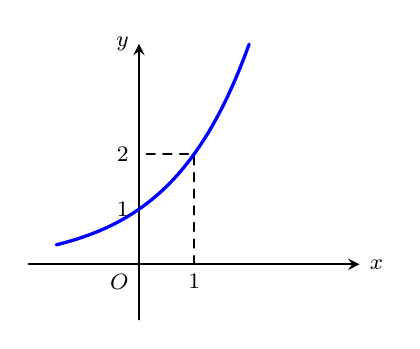
\begin{tikzpicture}[thick, font=\footnotesize, line cap=round, line join=round,scale=.7]
			\def\xmin{-2}
			\def\xmax{4}
			\def\ymin{-1}
			\def\ymax{4}
			\node[left] at (0,1) {$1$};
			\node[below] at (1,0) {$1$};
			\node[left] at (0,2) {$2$}; 
			\draw[-stealth] (\xmin,0)--(0,0)node[below left]{$O$}--(\xmax,0)node[right]{$x$};
			\draw[-stealth] (0,\ymin)--(0,\ymax)node[left]{$y$};
			\draw[dashed] (1,0)--(1,2)--(0,2);
			\draw[line width=1.2pt,color=blue,samples=200, domain=-1.5:2] plot (\x,{2^(\x)});
		\end{tikzpicture}
		}
		\loigiai{
		Đường cong trong hình bên là đồ thị của hàm số $y=a^x$, với $a>1$ và đồ thị hàm số đi qua điểm $A(1;2)$ nên ta chọn hàm số $y=2^x$.
		}
\end{ex}

%Cau8
\begin{ex}%[1D6H3-3]%[Dự án đề cương 3 khối NH 24-25-Dot 1- Nắng Đông]
	\immini{Đường cong trong hình bên là đồ thị của hàm số $y=\log_ax$, với $a>1$. Giá trị của biểu thức $T=a^4+25$ là
		\choice
		{$1321$}
		{\True $61$}
		{$41$}
		{$81$}}{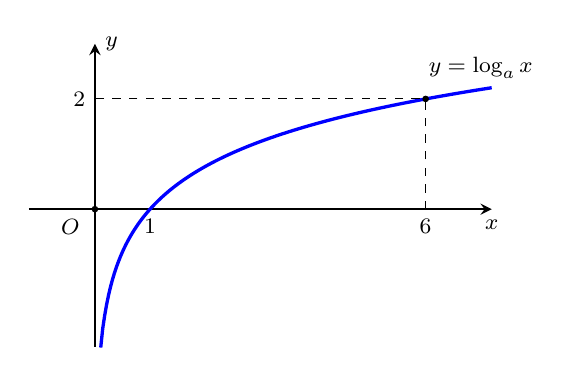
\begin{tikzpicture}[x=0.7 cm,y=0.7 cm,>=stealth,font=\footnotesize]
			\draw[->, color=black, thick] (-1.2,0) -- (7.2,0) node[below] {$x$};
			\draw[->,color=black,thick] (0,-2.5) -- (0,3) node[right]{$y$};
			\draw (-0.1,0) node[below left] {$O$};
			\draw[line width=1.2pt,color=blue,samples=200,domain=0.1054:7.2] plot (\x,{ln(\x)/ln(2.4494)});
			\draw (1,0) node[below]{$1$};
			\draw[dashed] (6,0) node[below]{$6$}--(6,2)--(0,2)node[left]{$2$};
			\draw (7,2.2) node[above]{$y=\log_ax$};
			\fill (6,2)circle(1.2pt) (0,0)circle(1.2pt);
	\end{tikzpicture}}
	\loigiai{Đồ thị hàm số $y=\log_ax$ đi qua điểm $B(6;2)$ nên $2=\log_a6 \Leftrightarrow a^2=6 \Leftrightarrow a=\sqrt{6}$ (vì $a>1$).\\
	Giá trị của biểu thức $T=a^4+25=36+25=61$. 
	}
\end{ex}

%Cau9
\begin{ex}%[1D6H3-2]%[Dự án đề cương 3 khối NH 24-25-Dot 1- Nắng Đông]
	\textit{(Trích đề thi GK2 - Trường THPT Thuận Thành 1-2-3 - Năm học 2024-2025)}\\
	Tập xác định của hàm số $y=\log_5(x-4)$ là
	\choice
	{\True $(4;+\infty)$}
	{$(-\infty;4)$}
	{$(5;+\infty)$}
	{$(-\infty;+\infty)$}
	\loigiai{
		Điều kiện xác định: $x-4>0 \Leftrightarrow x>4$ .\\
		Vậy tập xác định của hàm số đã cho là $\mathscr{D}=(4;+\infty)$ .}
\end{ex}

%Cau10
\begin{ex}% [1D6H3-2]%[Dự án đề cương 3 khối NH 24-25-Dot 1- Nắng Đông]
	\textit{(Trích đề thi GK2 - Trường THPT chuyên Nguyễn Đình Chiểu - Năm học 2024-2025)}\\
	Tập xác định của hàm số $y=\ln \left(-x^2+7x-10\right)$ là
	\choice
	{$(2;+\infty)$}
	{$[2;5]$}
	{$(5;+\infty)$}
	{\True $(2;5)$}
	\loigiai{
	Điều kiện xác định: $-x^2+7x-10>0\Leftrightarrow 2<x<5$. \\
	Vậy tập xác định của hàm số là $\mathscr{D}=(2;5)$.
	}
\end{ex}

%Cau11
\begin{ex}%[1D6H3-2]%[Dự án đề cương 3 khối NH 24-25-Dot 1- Nắng Đông]
	Có bao nhiêu số nguyên thuộc tập xác định của hàm số $y=\log \left[\left(26-x\right)\left(x+25\right)\right]$?
	\choice
	{\True $50$}
	{$52$}
	{$51$}
	{$53$}
	\loigiai{
		Điều kiện xác định: $\left(26-x\right)\left(x+25\right)>0\Leftrightarrow -25<x<26$.\\		
		Mà $x\in \mathbb{Z}\Rightarrow x\in \left\{-24;-23;-22;\ldots;25\right\}$.\\		
		Vậy có $50$ số nguyên thuộc tập xác định của hàm số đã cho.
	}
\end{ex}

%Cau12
\begin{ex}%[1D6H3-4]%[Dự án đề cương 3 khối NH 24-25-Dot 1- Nắng Đông]
	\textit{(Trích đề thi GK2 - Trường THPT chuyên Nguyễn Đình Chiểu - Năm học 2024-2025)}\\
	Với $b$, $c$ là hai số thực dương tuỳ ý thoả mãn $\log_5b\geq \log_5c$. Khẳng định nào dưới đây đúng?
	\choice
	{\True $b\geq c$}
	{$b\leq c$}
	{$b>c$}
	{$b<c$}
	\loigiai{
	Vì cơ số $5>1$ nên $\log_5b\geq \log_5c \Leftrightarrow b\geq c$.
	}
\end{ex}

%Cau13
\begin{ex}%[1D6H3-4]%[Dự án đề cương 3 khối NH 24-25-Dot 1- Nắng Đông]
	\textit{(Trích đề thi GK2 - Trường THPT Lương Ngọc Quyến - Năm học 2023-2024)}\\
	Cho $a,b>0$ thỏa mãn $a^{\tfrac{1}{2}}>a^{\tfrac{1}{3}}$, $b^{\tfrac{2}{3}}>b^{\tfrac{3}{4}}$. Khẳng định nào sau đây đúng?
	\choice
	{$0<a<1$, $0<b<1$}
	{$0<a<1$, $b>1$}
	{\True $a>1$, $0<b<1$}
	{$a>1$, $b>1$}
	\loigiai{
		Ta có $a^{\tfrac{1}{2}}>a^{\tfrac{1}{3}}$ và $\dfrac{1}{2}>\dfrac{1}{3}$ nên $a>1$.\\
		Lại có $b^{\tfrac{2}{3}}>b^{\tfrac{3}{4}}$ và $\dfrac{2}{3}<\dfrac{3}{4}$ nên $0<b<1$.}
\end{ex}

%Cau14
\begin{ex}%[1D6H3-3]%[Dự án đề cương 3 khối NH 24-25-Dot 1- Nắng Đông]
	\textit{(Trích đề thi GK2 - Trường THPT Lê Quý Đôn - Năm học 2023-2024)}
	\immini{Cho $3$ số $a$, $b$, $c>0$, $a \neq 1$, $b \neq 1$, $c \neq 1$. Đồ thị các hàm số $y=a^x$, $y=b^x$, $y=c^x$ được cho trong hình vẽ bên. Mệnh đề nào sau đây đúng?	
		\choice
		{$b<c<a$}
		{\True $a<c<b$}
		{$a<b<c$}
		{$c<a<b$}}{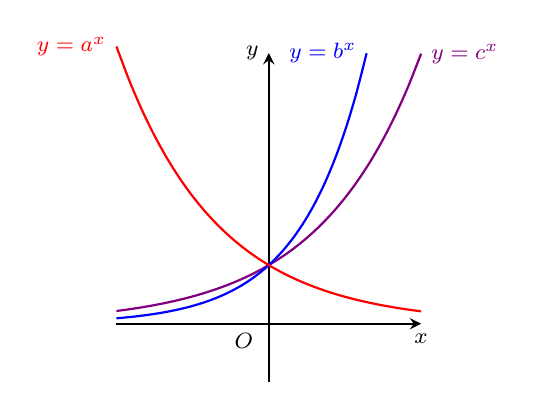
\begin{tikzpicture}[x=0.93cm,y=0.93cm,>=stealth,font=\footnotesize,scale=0.8]
			\draw[->, color=black, thick] (-2.6,0) -- (2.6,0) node[below] {$x$};
			\draw[->,color=black,thick] (0,-1) -- (0,4.62) node[left]{$y$};
			\draw (-0.1,0) node[below left] {$O$};
			\draw[smooth,violet,thick] plot[domain=-2.6:2.6](\x,{1.8^(\x)}) node [right]{$y=c^x$};
			\draw[smooth,blue,thick] plot[domain=-2.6:1.67](\x,{2.5^(\x)}) node [left]{$y=b^x$};		
			\draw[smooth,red,thick] plot[domain=2.6:-2.6](\x,{0.55^(\x)}) node [left]{$y=a^x$};
	\end{tikzpicture}}
	\loigiai{\immini{Vì đồ thị của hàm số $y=a^x$ có hướng đi xuống nên hàm số $y=a^x$ là hàm nghịch biến hay $0<a<1$.\\
			Vì đồ thị của hàm số $y=b^x$, $y=c^x$ có hướng đi xuống nên hàm số $y=b^x$, $y=c^x$ là hàm đồng biến hay $b,c>1$.\\
			Lấy điểm $B(1,y_B)$ thuộc đồ thị hàm số $y=b^x$. Khi đó $y_B=b$.\\
			Lấy điểm $C(1,y_C)$ thuộc đồ thị hàm số $y=c^x$. Khi đó $y_C=c$.\\
			Dựa vào hình vẽ ta được $y_B>y_C$ hay $b>c$. \\
			Vậy $0<a<1<c<b$ hay $a<c<b$.
		}{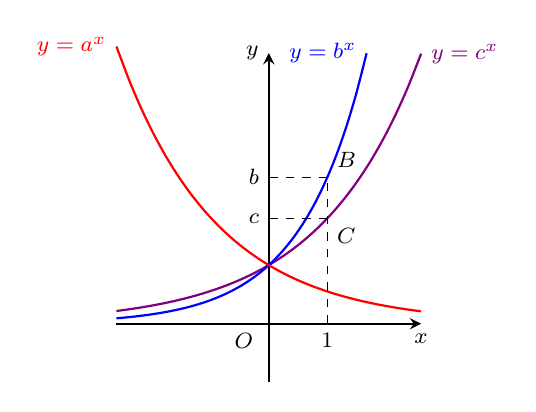
\begin{tikzpicture}[x=0.93cm,y=0.93cm,>=stealth,font=\footnotesize,scale=0.8]
				\draw[->, color=black, thick] (-2.6,0) -- (2.6,0) node[below] {$x$};
				\draw[->,color=black,thick] (0,-1) -- (0,4.62) node[left]{$y$};
				\draw (-0.1,0) node[below left] {$O$};
				\draw[smooth,violet,thick] plot[domain=-2.6:2.6](\x,{1.8^(\x)}) node [right]{$y=c^x$};
				\draw[smooth,blue,thick] plot[domain=-2.6:1.67](\x,{2.5^(\x)}) node [left]{$y=b^x$};		
				\draw[smooth,red,thick] plot[domain=2.6:-2.6](\x,{0.55^(\x)}) node [left]{$y=a^x$};
				\draw[dashed] (1,0)--(1,2.5) (1,1.8)--(0,1.8) (1,2.5)--(0,2.5);
				\draw (1,0) node[below]{$1$};
				\draw (0,1.8) node[left]{$c$};
				\draw (0,2.5) node[left]{$b$};
				\draw (1,2.5) node [above right]{$B$};
				\draw (1,1.8) node [below right]{$C$};
		\end{tikzpicture}}
	}
\end{ex}

%Cau15
\begin{ex}%[1D6H3-3]%[Dự án đề cương 3 khối NH 24-25-Dot 1- Nắng Đông]
	\textit{(Trích đề thi GK2 - Trường THPT Mạc Đĩnh Chi - Năm học 2023-2024)}
	\immini{Cho các hàm số $y=a^x$, $y=\log_bx$, $y=\log_cx$ có đồ thị như hình vẽ bên. Khẳng định nào sau đây \textbf{đúng}?
		\choice
		{\True $c>b>a$}
		{$b>a>c$}
		{$a>b>c$}
		{$b>c>a$}}{
		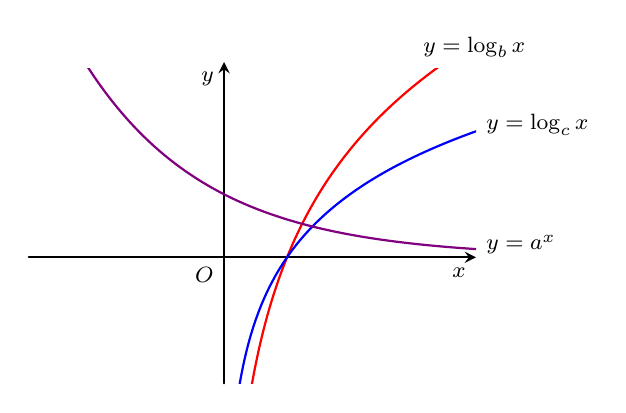
\begin{tikzpicture}[line join=round, line cap=round,>=stealth,thick,scale=0.8]
			\draw[->] (-3.1,0)--(4,0) node[below left] {\footnotesize $x$};
			\draw[->] (0,-2)--(0,3.1) node[below left] {\footnotesize$y$};
			\draw (0,0) node [below left] {\footnotesize $O$};
			\draw (4,2.1) node[right] {\footnotesize $y=\log_cx$};
			\draw (3,3) node[above right] {\footnotesize $y=\log_bx$};
			\draw (4,0.2) node[right] {\footnotesize $y=a^x$};
			\clip (-3,-2) rectangle (4,3);
			\draw[red,samples=200,domain=0.1:4,smooth,variable=\x] plot (\x,{log10((\x))/log10(1.5)});
			\draw[blue,samples=200,domain=0.1:4,smooth,variable=\x] plot (\x,{log10((\x))/log10(2)});
			\draw[violet,samples=200,domain=-3:4,smooth,variable=\x] plot (\x,{(0.6)^(\x)});
		\end{tikzpicture}
	}
	\loigiai{
		\immini{
			Dựa vào đồ thị ta có $y=a^x$ là của hàm số nghịch biến nên $a<1$.\\
			Đồ thị của $\log_b x$ và $\log_c x$ là của các hàm số đồng biến nên $b>1$, $c>1$.\\
			Kẻ đường thẳng $y=1$ như hình bên, ta có đường thẳng đó các đồ thị $y=\log_bx$ và $\log_cx$ tại các điểm có hoành độ lần lượt là $b$ và $c$.\\
			Dựa vào đó ta có $c>b>1>a$.}{
			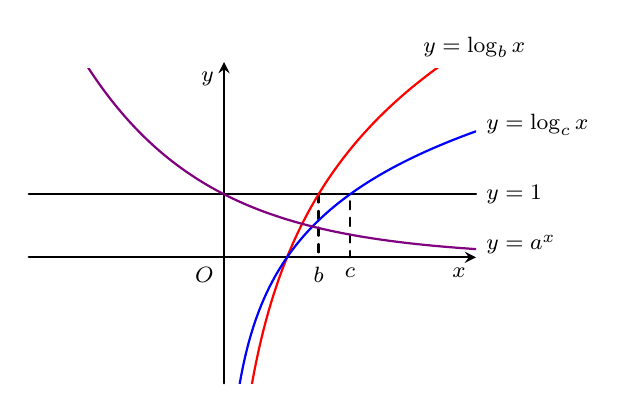
\begin{tikzpicture}[line join=round, line cap=round,>=stealth,thick,scale=0.8]
				\draw[->] (-3.1,0)--(4,0) node[below left] {\footnotesize $x$};
				\draw[->] (0,-2)--(0,3.1) node[below left] {\footnotesize$y$};
				\draw (0,0) node [below left] {\footnotesize $O$};
				\draw (4,2.1) node[right] {\footnotesize $y=\log_cx$};
				\draw (3,3) node[above right] {\footnotesize $y=\log_bx$};
				\draw (4,0.2) node[right] {\footnotesize $y=a^x$};
				\draw (-3.1,1)--(4,1) node[right] {\footnotesize $y=1$};
				\draw[dashed] (1.5,1)--(1.5,0) (0,1)--(2,1)--(2,0);
				\draw (1.5,0) node [below] {\footnotesize $b$};
				\draw (2,0) node [below] {\footnotesize $c$};
				\clip (-3,-2) rectangle (4,3);
				\draw[red,samples=200,domain=0.1:4,smooth,variable=\x] plot (\x,{log10((\x))/log10(1.5)});
				\draw[blue,samples=200,domain=0.1:4,smooth,variable=\x] plot (\x,{log10((\x))/log10(2)});
				\draw[violet,samples=200,domain=-3:4,smooth,variable=\x] plot (\x,{(0.6)^(\x)});
			\end{tikzpicture}
		}
	}
\end{ex}

%Cau16
\begin{ex}%[1D6H3-2]%[Dự án đề cương 3 khối NH 24-25-Dot 1- Nắng Đông]
	Có bao nhiêu giá trị nguyên của tham số $m$ để hàm số $y=\log_{0{,}5}\left(mx^2-mx+1\right)$ xác định $\forall x\in \mathbb{R}$?
	\choice
	{$3$}
	{\True $4$}
	{$2$}
	{$1$}
	\loigiai{
		Hàm số xác định $\forall x\in \mathbb{R}\Leftrightarrow mx^2-mx+1>0,\,\forall x\in \mathbb{R}.$ \hfill \qquad (*)\\
		Trường hợp 1: $ m=0 $,
		(*) trở thành $ 1>0,\,\forall x\in \mathbb{R} $ (đúng) nên $ m=0 $ thoả mãn.\\
		Trường hợp 2:
		(*) tương đương với $ \heva{&m>0\\&\Delta=m^2-4m<0}\Leftrightarrow \heva{&m>0\\&0<m<4.}$\\
		Vậy $0\le m<4$ thoả mãn đề bài hay có $4$ giá trị nguyên của tham số $m$ thoả yêu cầu.
	}
\end{ex}

%Cau17
\begin{ex}%[1D6H3-5]%[Dự án đề cương 3 khối NH 24-25-Dot 1- Nắng Đông]
	\textit{(Trích đề thi GK2 - Trường THPT chuyên Lê Quý Đôn - Năm học 2023-2024)}\\
	Ngân hàng thường tính lãi suất cho khách hàng theo thể thức lãi kép theo định kì, tức là nếu đến kì hạn người gửi không rút lãi ra thì tiền lãi được tính vào vốn của kì kế tiếp. Nếu một người gửi số tiền $P$ với lãi suất $r$ mỗi kì thì sau $n$ kì, số tiền người đó thu được (cả vốn lẫn lãi) được tính theo công thức lãi kép $P_n=P(1+r)^n$. Bác Châu gửi tiết kiệm số tiền $200$ triệu đồng kì hạn $12$ tháng với lãi suất $7\%$ một năm. Giả sử lãi suất không thay đổi, hỏi sau $4$ năm bác Châu lãnh được (cả vốn lẫn lãi) bao nhiêu triệu đồng? (kết quả làm tròn đến hàng đơn vị)
	\choice
	{$256$ triệu đồng}
	{$263$ triệu đồng}
	{\True $262$ triệu đồng}
	{$257$ triệu đồng}
	\loigiai{Theo đề ta có $P=200$, $r=0{,}07$, $n=4$.\\
		Số tiền bác Châu lãnh được sau $4$ năm là $$P_4=200(1+0{,}07)^4 \approx 262 \text{ (triệu đồng) }.$$
	}
\end{ex}
%cau18
\begin{ex}%[1D6H3-5]%[Dự án đề cương 3 khối NH 24-25-Dot 1- Nắng Đông]
	Độ $\mathrm{pH}$ của một dung dịch được tính theo công thức $\mathrm{pH}=-\log \left[H^{+}\right]$ trong đó $\left[H^{+}\right]$ là nồng độ ion $\left[H^{+}\right]$ của dung dịch đó tính bằng $\mathrm{mol}/$lít $\left(\mathrm{mol}/L\right)$. Biết rằng độ $\mathrm{pH}$ của một dung dịch bằng $2{,}44$, nồng độ ion $\left[H^{+}\right]$ của dung dịch đó bằng
	\choice
	{$3{,}7\cdot 10^{-5}$ mol/L}
	{\True $3{,}6\cdot 10^{-3}$ mol/L}
	{$3{,}2\cdot 10^{-4}$ mol/L}
	{$1{,}1\cdot 10^{-8}$ mol/L}
	\loigiai{Ta có $\mathrm{pH}=-\log \left[H^{+}\right]$ nên $2{,}44=-\log \left[H^{+}\right]$.\\
		Suy ra $\left[H^{+}\right]=10^{-2{,}44}\approx 3{,}6\cdot 10^{-3}$ mol/L.}
\end{ex}

%Cau19
\begin{ex}%[1D6V3-5]%[Dự án đề cương 3 khối NH 24-25-Dot 1- Nắng Đông]
	\textit{(Trích đề thi GK2 - Trường THPT chuyên Lương Thế Vinh - Năm học 2024-2025)} \\
	Cường độ một trận động đất $M$ (độ Richter) được cho bởi công thức $R=\log A-\log A_0$, với $A$ là biên độ rung chấn tối đa và $A_0$ là một biên độ chuẩn (hằng số). Đầu năm 2024, một trận động đất xảy ra ở Bắc Sulawesi, Indonesia có cường độ $8{,}7$ độ Richter. Trong cùng thời gian đó, một trận động đất khác ở Ishikawa, Nhật Bản có biên độ rung chấn tối đa mạnh hơn gấp $3$ lần trận động đất tại Indonesia. Hỏi cường độ của trận động đất ở Nhật bản là bao nhiêu? (kết quả được làm tròn đến hàng phần mười).
	\choice
	{$8{,}9$}
	{\True $9{,}2$}
	{$9{,}6$}
	{$10{,}2$}
	\loigiai{
		Gọi $M_1$, $M_2$ lần lượt là cường độ của trận động đất ở Indonesia và ở Nhật Bản.
		Trận động đất ở Indonesia có cường độ là $8{,}7$ độ Richter nên
		\allowdisplaybreaks
		\begin{eqnarray*}
			M_1=\log A-\log A_0 \Leftrightarrow 8{,}7=\log A-\log A_0.
		\end{eqnarray*}
		Trận động đất ở Nhật Bản có biên độ là $3A$, khi đó cường độ của trận động đất ở Nhật Bản là
		\allowdisplaybreaks
		\begin{eqnarray*}
			M_2=\log (3A)-\log A_0=\log 3+\left(\log A-\log A_0 \right)=\log 3+8{,}7\approx 9{,}2 \text{ (độ Richter)}.
		\end{eqnarray*}
	}
\end{ex}

%Cau20
\begin{ex}%[1D6V3-5]%[Dự án đề cương 3 khối NH 24-25-Dot 1- Nắng Đông]
	Sự tăng trưởng của một loài vi khuẩn C trong phòng thí nghiệm được tính theo công thức $S(t)=A\cdot \mathrm{e}^{rt}$, trong đó $A$ là số lượng vi khuẩn C ban đầu, $S(t)$ là số lượng vi khuẩn C có sau $t$ phút, $r$ là tỉ lệ tăng trưởng (với $r>0$) và $t$ là thời gian tăng trưởng (tính theo phút). Biết rằng số lượng vi khuẩn C ban đầu có $500$ con và sau $6$ giờ thì số lượng vi khuẩn C là $2\,000$ con. Hỏi sau $20$ giờ kể từ lúc bắt đầu thì số lượng vi khuẩn C là bao nhiêu con? (làm tròn đến hàng đơn vị)
	\choice
	{\True $50\,797$ con}
	{$50\,779$ con}  
	{$57\,097$ con}  
	{$57\,970$ con} 
	\loigiai{
		Số lượng vi khuẩn C ban đầu là $A=500$ (con).\\
		Theo đề, ta có 
		\begin{eqnarray*}
			&&S(360)=2\,000\\
			&\Leftrightarrow&500\cdot \mathrm{e}^{360r}=2\,000\\
			&\Leftrightarrow&\mathrm{e}^{360r}=4\\
			&\Leftrightarrow&360r=\ln 4\\
			&\Leftrightarrow&r=\dfrac{\ln 4}{360}.
		\end{eqnarray*}
		Số vi khuẩn C sau $20$ giờ (tức $1\,200$ phút) là
		\begin{eqnarray*}
			&S(1\,200)&=500\cdot \mathrm{e}^{1\,200r}\\
			&&=500\cdot \mathrm{e}^{1\,200\cdot \tfrac{\ln 4}{360}}\\
			&&\approx 50\,797.
		\end{eqnarray*}
	Vậy sau $20$ giờ kể từ lúc bắt đầu thì số lượng vi khuẩn C là $50\,797$ con.
 	}
\end{ex}


\Closesolutionfile{ans}

\ind{PHẦN II.} \inden{Câu trắc nghiệm đúng sai. Trong mỗi ý a), b), c), d) ở mỗi câu, học sinh chọn đúng hoặc sai.}\\
\setcounter{ex}{0}
\Opensolutionfile{ans}[ans/2D1-Bai1-DS]%--Đặt tên 2D1-Bai1-DS
%Cau1
\begin{ex}%[1D6H3-3]%[Dự án đề cương 3 khối NH 24-25-Dot 1- Nắng Đông]
	Xét hàm số $f(x)=2^x$ trên tập số thực $\mathbb{R}$. Khi đó
	\choiceTF
	{Đồ thị hàm số $f(x)$ luôn đi qua điểm $A(1;0)$}
	{\True Hàm số $f(x)$ có tập xác định là $\mathbb{R}$}
	{Hàm số $f(x)$ nghịch biến trên khoảng $(-\infty;+\infty)$}
	{Có đúng $6$ số nguyên dương của $x$ để $f(x)\leq 32$}
	\loigiai{
		\begin{itemchoice}
			\itemch Do $2^1=2$ nên đồ thị hàm số $f(x)$ không đi qua điểm $A(1;0)$.
			\itemch Hàm số $f(x)=2^x$ có tập xác định là $\mathbb{R}$.
			\itemch Hàm số $f(x)=2^x$ đồng biến trên khoảng $(-\infty;+\infty)$ vì có cơ số là $2>1$.
			\itemch Ta có $f(x)\leq 32\Leftrightarrow 2^x\leq 32\Leftrightarrow 2^x\leq 2^5 \Leftrightarrow x\leq 5$ nên có đúng $5$ số nguyên dương của $x$ để $f(x)\leq 32$.
		\end{itemchoice}
	}
\end{ex}

%Cau2
\begin{ex}%[1D6H3-3]%[Dự án đề cương 3 khối NH 24-25-Dot 1- Nắng Đông]
	Hình vẽ dưới đây là đồ thị của các hàm số mũ $y=a^x$, $y=b^x$, $y=c^x$, với $a$, $b$, $c$ là ba số thực dương khác $1$.
	\begin{center}
		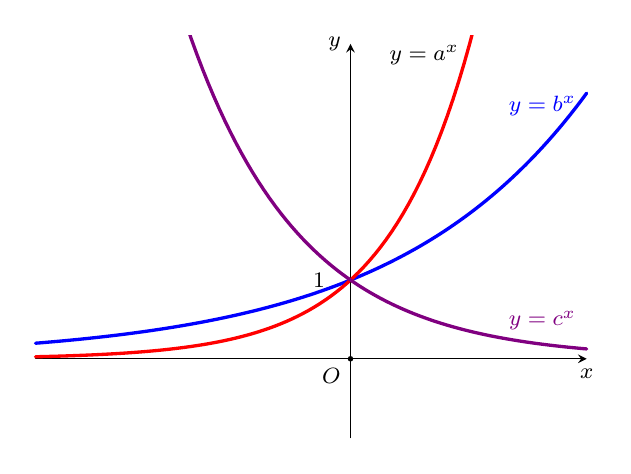
\begin{tikzpicture}[scale=1, font=\footnotesize, line join=round, line cap=round,>=stealth]
			\def\xmin{-4};\def\ymin{-1};\def\xmax{3};\def\ymax{4};
			\coordinate (O) at (0,0);
			\draw[->] (\xmin,0)--(\xmax,0) node[below]{$x$};
			\draw[->] (0,\ymin)--(0,\ymax) node[left]{$y$};
			\fill (O) node[below left]{$O$} circle(1pt);
			\clip ({\xmin-0.1},{\ymin-0.1}) rectangle ({\xmax+0.1},{\ymax+0.1});
			\foreach \y in {1}{
				\fill (0,\y) node[left=2mm]{$\y$} circle(1pt);
			}
			\draw[line width=1.2pt,color=blue,samples=100] plot[domain=-4:3](\x,{pow(1.5,(\x))}) node[below left=-1mm,xshift=-1mm] {$y=b^x$};
			\draw[line width=1.2pt,color=red,samples=100] plot[domain=-4:3](\x,{pow(2.5,(\x))});
			\path (1.5,{pow(2.5,1.5)}) node[left,yshift=-1mm] {$y=a^x$};
			\draw[line width=1.2pt,color=violet,samples=100] plot[domain=-4:3](\x,{pow(0.5,(\x))})
			node[above left=-1mm,xshift=-1mm,yshift=2mm] {$y=c^x$};
			
		\end{tikzpicture}
	\end{center}
	\choiceTF
	{\True Hàm số $y=a^x$ đồng biến trên $\mathbb{R}$}
	{\True Hàm số $y=c^x$ nghịch biến trên $\mathbb{R}$}
	{$b<c$}
	{\True $a>b>1>c>0$}
	\loigiai
	{\begin{itemchoice}
			\itemch Dựa vào đồ thị ta được hàm số $y=a^x$ đồng biến trên $\mathbb{R}$ hay $a>1$.
			\itemch Dựa vào đồ thị ta được hàm số $y=c^x$ nghịch biến trên $\mathbb{R}$ hay $0<c<1$.
			\itemch Dựa vào đồ thị ta được hàm số $y=b^x$ đồng biến trên $\mathbb{R}$ hay $b>1$.\\
			Suy ra $b>c$.  
			\itemch Với $x>0$ thì $a^x>b^x$ nên suy ra $a>b$. Hay $a>b>1>c>0$.
		\end{itemchoice}
	}
\end{ex}
%Cau3
\begin{ex}%[1D6H3-3]%[Dự án đề cương 3 khối NH 24-25-Dot 1- Nắng Đông]
	\textit{(Trích đề thi GK2 - Trường THPT Kim Sơn A - Năm học 2023-2024)} \\
	Cho hàm số $y=f(x)=\log _{2}x$, với $x>0$ có đồ thị $(C)$.
	\choiceTF
	{\True Tập xác định của hàm số $y=f(x)=\log _{2}x$ là $\mathscr{D}=(0 ;+\infty)$}
	{Hàm số $y=f(x)=\log _{2}x$ đồng biến trên $\mathbb{R}$}
	{\True Đồ thị $(C)$ đi qua điểm $(4;2)$}
	{Tổng $T=f\left(\dfrac{1}{2}\right)+f\left(\dfrac{2}{3}\right)+f\left(\dfrac{3}{4}\right)+\ldots+f\left(\dfrac{63}{64}\right)=6$}
	\loigiai{
		\begin{itemchoice}
			\itemch Điều kiện xác định: $x>0$ nên hàm số có tập xác định là $\mathscr{D}=(0;+\infty)$.
			\itemch Vì cơ số $2>1$ nên hàm số đồng biến trên khoảng $(0 ;+\infty)$.
			\itemch Ta có $x=4 \Rightarrow y=\log_22=2$, nên đồ thị hàm số $(C)$ đi qua điểm $(4;2)$. 
			\itemch Ta có 	
			\allowdisplaybreaks \vspace*{-0.7cm}
			\begin{eqnarray*} 
				T &= &  f\left(\dfrac{1}{2}\right)+f\left(\dfrac{2}{3}\right)+f\left(\dfrac{3}{4}\right)+\ldots+f\left(\dfrac{63}{64}\right)\\
				& = & \log_2 1 -\log_2 2  + \log_2 2 -\log_2 3 +\ldots + \log_2 63 -\log_2 64\\
				& = & 0 - \log_2 64 = -6.
			\end{eqnarray*}
		\end{itemchoice}
	}
\end{ex}

%Cau4
\begin{ex}%[1D6H3-2]%[Dự án đề cương 3 khối NH 24-25-Dot 1- Nắng Đông]
	Cho hai hàm số $f(x)=\ln{\left(x^{2026}+1\right)}$ và $g(x)=3^{x^2+1}$. 
	\choiceTF
	{Hàm số $f(x)$ có tập xác định là $(0;+\infty)$}
	{\True Hàm số $f(x)$ có tập giá trị là $[0;+\infty)$}
	{\True Hàm số $g(x)$ có tập xác định là $\mathbb{R}$}
	{\True Hàm số $g(x)$ có tập giá trị là $[3;+\infty)$}
	\loigiai{
		\begin{itemchoice}
			\itemch Điều kiện xác định: $x^{2026}+1>0 \Leftrightarrow \forall x\in \mathbb{R}$.
			\itemch Với $x\in \mathbb{R}$ thì $x^{2026}+1\geq 1$ nên $\ln{\left(x^{2026}+1\right)} \geq 0$. Hay hàm số $f(x)=\ln{\left(x^{2026}+1\right)}$ có tập giá trị là $[0;+\infty)$.
			\itemch Vì $x^2+1$ có nghĩa với mọi $x\in \mathbb{R}$ nên hàm số $g(x)=3^{x^2+1}$ có tập xác định là $\mathbb{R}$.
			\itemch Với $x\in \mathbb{R}$ thì $x^2+1\geq 1$ nên $3^{x^2+1}\geq 3$ hay hàm số $g(x)=3^{x^2+1}$ có tập giá trị là $[3;+\infty)$.
		\end{itemchoice}
	}
\end{ex}
%Cau5
\begin{ex}%[1D6V3-5]%[Dự án đề cương 3 khối NH 24-25-Dot 1- Nắng Đông]
	Ông Dũng gửi số tiền $500$ triệu đồng vào ngân hàng A với lãi suất $0,5\% / \mbox{tháng}$. Biết rằng nếu không rút tiền ra khỏi ngân hàng thì cứ sau mỗi tháng, số tiền lãi sẽ được nhập vào vốn ban đầu. Trong suốt quá trình gửi thì ông Dũng không rút tiền ra và lãi suất cũng không thay đổi. (đơn vị: triệu đồng và kết quả làn tròn đến hàng phần chục)
	\choiceTF
	{\True Sau đúng $5$ tháng, ông Dũng lãnh được số tiền là $512{,}6$ triệu đồng}
	{\True Sau đúng $1$ năm, ông Dũng lãnh được số tiền là $530{,}8$ triệu đồng}
	{Ông Dũng muốn lãnh được số tiền là $600$ triệu đồng thì thời gian ông phải gửi là đúng $3$ năm}
	{\True Để lãnh được số tiền gấp đôi số tiền gốc ban đầu thì ông Dũng phải gửi ngân hàng ít nhất là $139$ tháng}
	\loigiai{
		Theo đề ta có $P=500$, $r=0{,}005$.
		\begin{itemchoice}
			\itemch Số tiền ông Dũng được lãnh sau đúng $5$ tháng là $P_5=500(1+0{,}005)^5 \approx 512{,}6$ (triệu đồng).
			\itemch Số tiền ông Dũng được lãnh sau đúng $1$ năm là $P_{12}=500(1+0{,}005)^{12} \approx 530{,}8$ (triệu đồng).
			\itemch Số tiền ông Dũng được lãnh sau đúng $3$ năm là $P_{36}=500(1+0{,}005)^{36} \approx 598{,}3$ (triệu đồng).\\ Hay để lãnh được số tiền là $600$ triệu đồng thì ông Dũng phải gửi hơn $3$ năm.
			\itemch Số tiền ông Dũng được lãnh sau đúng $139$ tháng là $P_{139}=500(1+0{,}005)^{139} \approx 1\,000{,}1$ (triệu đồng).\\ Hay ông Dũng lãnh được số tiền gấp đôi số tiền gốc ban đầu.
		\end{itemchoice}
	}
\end{ex} 
\Closesolutionfile{ans}


\ind{PHẦN III.} \inden{Câu trắc nghiệm trả lời ngắn.}\\
\setcounter{ex}{0}
\Opensolutionfile{ans}[ans/2D1-Bai1-TLN]%--Đặt tên 2D1-Bai1-DS

%Cau1
\begin{ex}%[1D6H3-2]%[Dự án đề cương 3 khối NH 24-25-Dot 1- Nắng Đông]
	Cho hàm số $y=f(x)=3^{\sqrt{11-x}}+\dfrac{2x-1}{x^2-4}$ có tập xác định $\mathscr{D}0$. Hỏi tập $\mathscr{D}$ có bao nhiêu số nguyên lớn hơn $-24$? 
	\shortans[oly]{33}
	\loigiai{Điều kiện xác định: $\heva{&11-x\geq 0\\&x^2-4\ne 0}\Leftrightarrow \heva{&x\leq 11\\&x\ne \pm 2}$.\\
	Suy ra $\mathscr{D}=(-\infty;11]\setminus \{-2;2\}$.\\
	Mà $x\in \mathscr{D}$ và $x>-24$ nên ta được $x\in \{-23;-22;\ldots;-3;-1;0;1;3;4;\ldots;11\}$.\\
	Vậy có $33$ số nguyên thuộc $\mathscr{D}$ thoả yêu cầu.
	}
\end{ex}
%cau2
\begin{ex}%[1D6H3-5]%[Dự án đề cương 3 khối NH 24-25-Dot 1- Nắng Đông]
	Ông An gửi số tiền $700$ triệu đồng vào ngân hàng với lãi suất $7\%$ một năm, biết rằng nếu không rút tiền ra khỏi ngân hàng thì cứ sau mỗi năm, số tiền lãi sẽ được nhập vào vốn ban đâu. Sau thời gian $7$ năm nếu không rút lãi lần nào thì số tiền mà ông An nhận được tính cả gốc và lãi là bao nhiêu triệu đồng? Biết ngân hàng không thay đổi lãi suất trong suốt thời gian ông An gửi. (kết quả làm tròn đến hàng đơn vị).
	\shortans[oly]{1124}
	\loigiai{Theo đề ta có $P=700$, $r=0{,}07$, $n=7$.\\
		Số tiền ông An nhận được sau đúng $7$ năm là $P_7=700(1+0{,}07)^7 \approx 1\,124$ (triệu đồng).
	}
\end{ex}
%Cau3
\begin{ex}%[1D6V3-5]%[Dự án đề cương 3 khối NH 24-25-Dot 1- Nắng Đông]
	Theo số liệu của Tổng cục thống kê, năm $2016$ dân số Việt Nam ước tính $94\,444\,200$ người. Tỉ lệ tăng dân số hàng năm ở Việt Nam được duy trì ở mức $1{,}07\%$. Cho biết sự tăng dân số được tính theo công thức $S=A\cdot \mathrm{e}^{Nr}$ (trong đó $A$ là dân số của năm lấy làm mốc tính, $S$ là dân số sau $N$ năm, $r$ là tỉ lệ tăng dân số hàng năm). Cứ tăng dân số với tỉ lệ như vậy thì đến năm nào, dân số nước ta ở mức $120$ triệu người?
	\shortans[oly]{2039}
	\loigiai{
		Gọi $n$ là số năm để dân số đạt mức $120$ triệu người tính mốc từ năm $2016$.\\
		Ta có $120\,000\,000=94\,444\,200\mathrm{e}^{n\cdot0{,}0107}\Rightarrow n\approx \dfrac{\ln 1{,}27}{0{,}0107}\approx 22{,}34$.\\
		Vậy trong năm thứ $23$ (tức là năm $2\,016+23=2\,039$) thì dân số đạt mức $120$ triệu người.
	}
\end{ex}
%Cau4
\begin{ex}%[1D6V3-5]%[Dự án đề cương 3 khối NH 24-25-Dot 1- Nắng Đông]
	Sự tăng trưởng của loại vi khuẩn tuân theo công thức $S=A \mathrm{e}^{rt}$, trong đó $A$ là số lượng vi khuẩn ban đầu, $r$ là tỉ lệ tăng trưởng ($r>0$), $t$ là thời gian tăng trưởng (tính theo đơn vị là giờ). Biết số vi khuẩn ban đầu là $100$ con và sau $5$ giờ có $300$ con. Thời gian để vi khuân tăng gấp đôi ban đầu là bao nhiêu giờ? (kết quả làm tròn đến hàng phần trăm).
	\shortans[oly]{3{,}15}
	\loigiai{
		Ta có $300=100\mathrm{e}^{5r}\Leftrightarrow e^{5r}=3\Leftrightarrow 5r=\ln 3\Leftrightarrow r=\dfrac{\ln 3}{5}$.\\
		Theo yêu cầu bài toán ta lại có $$200=100\mathrm{e}^{rt}\Leftrightarrow e^{rt}=2\Leftrightarrow rt=\ln 2 \Leftrightarrow t=\dfrac{5\ln 2}{\ln 3}\approx 3{,}15 \, (\text{h})$$
	}
\end{ex}
%Cau5
\begin{ex}%[1D6V3-3]%[Dự án đề cương 3 khối NH 24-25-Dot 1- Nắng Đông]
	\immini{\hfill\\
		Cho hàm số $y=\log_a x$ và $y=\log_b x$ có đồ thị như hình vẽ bên, với $a$, $b$ là hai số thực lớn hơn $1$. Đường thẳng $x=9$ cắt trục hoành, đồ thị hàm số $y=\log_a x$ và $\log_b x$ lần lượt tại $H,M$ và $N$. Biết rằng $HM=MN$. Khi đó tính giá trị của biểu thức $T=25\log_ab^2+26\log_ba^3$.
	}{
		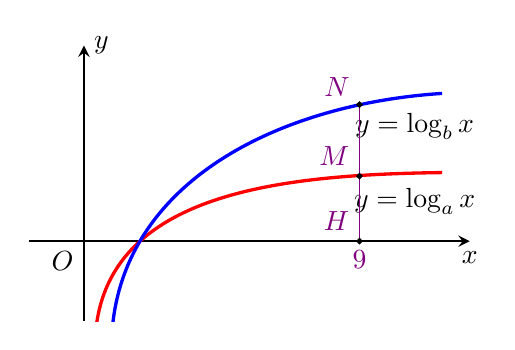
\begin{tikzpicture}[scale=0.7,thick,>=stealth]
			\draw[->](-1,0.95)--++(0:8)node[below]{$x$};
			\draw[->](0,-0.5)--++(90:5)node[right]{$y$};
			\node[below] at (6,2.1) {\normalsize{$y=\log_ax$}};
			\node[below] at (6,3.45) {\normalsize{$y=\log_bx$}};
			\clip(-1,-0.5)rectangle(6.5,4);
			\draw[line width=1.2pt,color=red] (0.2,-1) to [out=90, in=180] (8,2.2);
			\draw[line width=1.2pt,color=blue] (0.5,-1) to [out=90, in=170] (9,3.5 );
			\node[below left] at (0,0.95) {$O$};
			\draw[thin,violet] (5,0.95)node[below]{$9$}--(5,3.4)node[above left]{$N$};
			\node[above left,violet] at (5,0.96) {$H$};
			\node[above left,violet] at (5,2.13){$M$};
			\filldraw (5,0.95) circle(1pt);  
			\filldraw (5,2.13) circle(1pt);
			\filldraw (5,3.43) circle(1pt); 
		\end{tikzpicture}
	}
	\shortans[oly]{181}
	\loigiai{
		Ta có $\heva{& HM=y_{M}=\log_a9\\& MN=y_N-y_M=\log_b9-\log_a9}.$\\
		Vì $HM=MN$ nên $\log_a 9=\log_b 9-\log_a9\Leftrightarrow\log_{\sqrt{a}}9=\log_b9\Leftrightarrow a=b^2$.\\
		Vậy $T=25\log_ab^2+26\log_ba^3=25\log_{b^2}b^2+26\log_bb^6=25\cdot 1+26\cdot6=181$.
	}
\end{ex}

\Closesolutionfile{ans}


\ind{PHẦN IV.} \inden{Tự luận.}\\
\setcounter{ex}{0}
%Cau1

\begin{ex}%[1D6H3-3]%[Dự án đề cương 3 khối NH 24-25-Dot 1- Nắng Đông]
	Khảo sát sự biến thiên và vẽ đồ thị các hàm số sau
	\begin{multicols}{2}
		\begin{enumerate}
			\item $y=2^x$;
			\item $y=\log_{\tfrac{1}{4}}x$.
		\end{enumerate}
	\end{multicols}
	\loigiai{
		\begin{enumerate}
			\item Tập xác định $\mathscr{D}=\mathbb{R}$.\\
				Vì hàm số $y=2^x$ có cơ số $2>1$ nên hàm số $y=2^x$ đồng biến trên $\mathbb{R}$, ta có bảng biến thiên như sau
				\begin{center}
					
\begin{tikzpicture}[>=stealth,line join=round,line cap=round,font=\footnotesize]
						\tkzTabInit[nocadre=false,lgt=2,espcl=2,deltacl=0.5]{$x$/0.7,$y=2^x$/2}
						{$-\infty$ , $0$ , $+\infty$}
						\tkzTabVar{-/$0$ , R , +/$+\infty$}
						\tkzTabIma{1}{3}{2}{$1$}% Từ cột 1 đến cột 3 đặt f(2) tại cột 2.
					\end{tikzpicture}
				\end{center}
				Bảng giá trị
				\begin{center}
					\begin{tabular}{|c|c|c|c|c|}
						\hline
						$x$  & $-1$ & $0$ & $1$ & $2$ \\
						\hline
						$y=3^{x}$& $\dfrac{1}{2}$ & $1$ & $2$ & $4$ \\
						\hline
					\end{tabular}
				\end{center}
				Đồ thị của hàm số $y=3^x$ là một đường cong liền nét đi qua các điểm $A\left(-1;\dfrac{1}{2}\right)$, $B(0;1)$, $C(1;2)$, $D(2;4)$.
				\begin{center}
					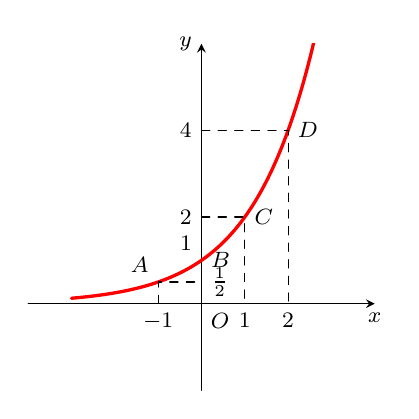
\begin{tikzpicture}[>=stealth,line join=round,line cap=round,font=\footnotesize,scale=0.55]
					\def\a{2}
					\draw[->] (-4,0) -- (4,0) node[below] {$x$};
					\draw[->] (0,-2) -- (0,6) node[left] {$y$};
					\draw (0,0)node[below right=-0.1]{$O$};
					\clip (-4,-2)rectangle(4,6);
					\draw[line width=1.2pt,color=red,samples=200,smooth,domain=-3:4] plot(\x, {\a^\x});
					\draw[dashed] (0,2)--(1,2) node[right]{$C$}--(1,0);
					\draw[dashed] (0,4)--(2,4)node[right]{$D$}--(2,0);
					\draw[dashed] (-1,0)--(-1,1/2)node[above left]{$A$}--(0,1/2)node[right]{$\frac{1}{2}$};
					\draw (0,1) node [above left=-0.1] {$1$}node[right]{$B$};
					\draw (1,0) node [below] {$1$};
					\draw (0,2) node [left] {$2$};
					\draw (2,0) node [below] {$2$};
					\draw (0,4) node [left] {$4$};
					\draw (-1,0) node [below] {$-1$};
					\end{tikzpicture}
				\end{center}

			\item Tập xác định $\mathscr{D}=(0;+\infty)$.\\
			Vì hàm số $y=\log_{\tfrac{1}{4}} x$ có cơ số $\dfrac{1}{4}<1$ nên hàm số $y=\log_{\tfrac{1}{4}} x$ nghịch biến trên khoảng $(0;+\infty)$, ta có bảng biến thiên như sau
			\begin{center}
				
\begin{tikzpicture}[>=stealth,line join=round,line cap=round,font=\footnotesize]
					\tkzTabInit[nocadre=false,lgt=2.3,espcl=2,deltacl=0.5]{$x$/0.7,$y=\log_{\tfrac{1}{4}}x$/2}
					{$0$ , $1$ , $+\infty$}
					\tkzTabVar{+/$+\infty$ , R , -/$-\infty$}
					\tkzTabIma{1}{3}{2}{$0$}% Từ cột 1 đến cột 3 đặt f(2) tại cột 2.
				\end{tikzpicture}
			\end{center}
			Bảng giá trị
			\begin{center}
				\begin{tabular}{|c|c|c|c|}
					\hline
					$x$ & $\dfrac{1}{4}$  & $1$ & $4$ \\
					\hline
					$y=\log_{\tfrac{1}{4}}x$ & $1$ & $0$ & $-1$\\
					\hline
				\end{tabular}
			\end{center}
			Đồ thị của hàm số $y=\log_3 x$ là một đường cong liền nét đi qua các điểm $H\left(\dfrac{1}{4};1\right)$, $E(1;0)$, $F(4;-1)$.
			\begin{center}
				\begin{tikzpicture}[>=stealth,line join=round,line cap=round,font=\footnotesize,scale=0.9]
					\draw[->] (-1,0)--(5,0) node[right] {$x$};
					\draw[->] (0,-2)--(0,2) node[above] {$y$};
					\draw [line width=1.2pt,color=blue,smooth,domain=0.065:5,samples=100]plot(\x,{(ln(\x))/(ln(0.25))});
					\draw[dashed] (4,0)--(4,-1)node[below]{$F$}--(0,-1) (0.25,0)--(0.25,1)node[right]{$H$}--(0,1);
					\fill (0,0)node[above left]{\footnotesize{$O$}}circle(1.2pt) (1,0)node[below]{\footnotesize{$1$}}circle(1.2pt) (4,0)node[above]{\footnotesize{$4$}}circle(1.2pt) (0.25,0)node[below]{\footnotesize{$\tfrac{1}{4}$}}circle(1.2pt) (0,1)node[left]{\footnotesize{$1$}}circle(1.2pt) (0,-1)node[left]{\footnotesize{$-1$}}circle(1.2pt)  (4,-1)circle(1.2pt) (0.25,1)circle(1.2pt);
					\path (1,0)node[above]{$E$};
				\end{tikzpicture}
			\end{center}
		\end{enumerate}}
\end{ex}

%Cau2
\begin{ex}%[1D6H3-2]%[Dự án đề cương 3 khối NH 24-25-Dot 1- Nắng Đông]
	Tìm tập xác định hàm số sau
	\begin{multicols}{2}
		\begin{enumerate}
			\item $y=7^{\sqrt{-x^2+5 x-4}}$;
			\item) $y=\log _2(2 x-8)$.
		\end{enumerate}
	\end{multicols}
	
	\loigiai{
		\begin{enumerate}
			\item Điều kiện xác định: $-x^2+5 x-4\ge 0\Leftrightarrow 1\le x\le 4$.\\
			Vậy tập xác định của hàm số đã cho là $\mathscr{D}=\left[1;4\right]$.
			\item Điều kiện xác định: $2 x-8\Leftrightarrow x>4$.\\
			Vậy tập xác định của hàm số đã cho là $\mathscr{D}=(4;+\infty)$.
		\end{enumerate}
	}
\end{ex}
%Cau3
\begin{ex}%[1D6H3-5]%[Dự án đề cương 3 khối NH 24-25-Dot 1- Nắng Đông]
	Trong một nghiên cứu, một nhóm học sinh được cho xem cùng một danh sách các loài động vật và được kiểm tra lại xem họ còn nhớ bao nhiêu phần trăm danh sách đó sau mỗi tháng. Giả sử sau $t$ tháng, khả năng nhớ trung bình của nhóm học sinh đó được tính theo công thức $M(t) = 75 - 20 \ln (t+1)$, $0 \leq t \leq 12$ (đơn vị: \%). Hãy tính khả năng nhớ trung bình của nhóm học sinh đó sau $6$ tháng (làm tròn đến hàng phần chục).
	\loigiai{
		Khả năng nhớ trung bình của nhóm học sinh đó sau $6$ tháng là $$M(6) = 75 - 20 \ln (6+1) \approx 36{,}1 \%.$$
	}
\end{ex}

%cau5
\begin{ex}%[1D6H3-5]%[Dự án đề cương 3 khối NH 24-25-Dot 1- Nắng Đông]
	Giả sử một chất phóng xạ bị phân rã theo cách sao cho khối lượng $m(t)$ của chất còn lại (tính bằng kilôgam) sau $t$ ngày được cho bởi hàm số $m(t) = 13 \mathrm{e}^{-0,0015t}$.
	\begin{enumerate}
		\item Tìm khối lượng của chất đó tại thời điểm $t = 0$;
		\item Sau $45$ ngày khối lượng chất đó còn lại là bao nhiêu?
	\end{enumerate}
	\loigiai{
		\begin{enumerate}
			\item Ta có $m(0) = 13\mathrm e^{0} = 13$ (kilôgam).
			\item Ta có $m(45) = 13\mathrm e^{-0,015 \cdot 45} \approx 6{,}62$ (kilôgam).
		\end{enumerate}
	}
\end{ex}

%Cau6
\begin{ex}%[1D6H3-3]%[Dự án đề cương 3 khối NH 24-25-Dot 1- Nắng Đông]
	Tìm tập giá trị của các hàm số sau
	\begin{multicols}{2}
		\begin{enumerate}
			\item $y=2^{x^2+3}$;
			\item $y=\log_3{\left(3+|x|\right)}$;
		\end{enumerate}
	\end{multicols}
	\loigiai{
		\begin{enumerate}
			\item Tập xác định của hàm số $y=2^{x^2+3}$ là $\mathscr{D}=\mathbb{R}$.\\
			Với $x\in \mathscr{D}$ thì $x^2+3\geq 3\Leftrightarrow 2^{x^2+3}\geq 2^3$ hay $y\geq 8$.\\
			Vậy tập giá trị của hàm số đã cho là $T=[8;+\infty)$.
			\item Điều kiện xác định: $3+|x|>0\Leftrightarrow x\in \mathbb{R}$.\\
			Suy ra tập xác định của hàm số $y=\log_3{\left(3+|x|\right)}$ là $\mathscr{D}=\mathbb{R}$.\\
			Với $x\in \mathscr{D}$ thì $3+|x|\geq 3\Leftrightarrow \log_3{\left(3+|x|\right)}\geq \log_33$ hay $y\geq 1$.\\
			Vậy Vậy tập giá trị của hàm số đã cho là $T=[1;+\infty)$.
		\end{enumerate}
	}
\end{ex}

%Cau7
\begin{ex}%[1D6H3-5]%[Dự án đề cương 3 khối NH 24-25-Dot 1- Nắng Đông]
	Các nhà tâm lí học sử dụng mô hình hàm số mũ để mô phỏng quá trình học tập của một học sinh như sau: $f(t)=c\left(1-\mathrm{e}^{-k t}\right)$, trong đó $c$ là tổng số đơn vị kiến thức học sinh phải học, $k$ (kiến thức/ngày) là tốc độ tiếp thu của học sinh, $t$ (ngày) là thời gian học và $f(t)$ là số đơn vị kiến thức học sinh đã học được.
	\begin{center}
		(\textit{Nguồn:} R.I. Charles et al., Algebra 2, Pearson)
	\end{center}
	 Giả sử một em học sinh phải tiếp thu $25$ đơn vị kiến thức mới. Biết rằng tốc độ tiếp thu của em học sinh là $k=0{,}2$. Hỏi em học sinh sẽ nhớ được (khoảng) bao nhiêu đơn vị kiến thức mới sau $2$ ngày? Và sau $8$ ngày?
	\loigiai{
		Số đơn vị kiến thức mới em học sinh sẽ nhớ sau $2$ ngày là
		$$f(2)=25\left(1-\mathrm{e}^{-0{,}2\cdot2}\right)\approx 8{,}24\text{ (đơn vị)}.$$
		Số đơn vị kiến thức mới em học sinh sẽ nhớ sau $8$ ngày là
		$$f(8)=25\left(1-\mathrm{e}^{-0{,}2\cdot8}\right)\approx 19{,}95\text{ (đơn vị)}.$$
	}	
\end{ex}
%Cau7
\begin{ex}%[1D6H3-3]%[Dự án đề cương 3 khối NH 24-25-Dot 1- Nắng Đông]
	Gọi $S$ là tập hợp tất cả các số nguyên dương $a$ để hàm số mũ $y=\left(2026-a^2\right)^x$ đồng biến trên $\mathbb{R}$. Tính tổng các phần tử của tập $S$.
	\loigiai{
		Đề hàm số $y=\left(2026-a^2\right)^x$ đồng biến trên $\mathbb{R}$ thì $2026-a^2>1\Rightarrow a^2<2025\Rightarrow -45<a<45$.\\
		Vì $a \in \mathbb{Z^+}$ nên $a\in \{1;2;3;\ldots;45\}$.\\
		Suy ra $S=\{1;2;3;\ldots;45\}$.\\
		Vậy tổng các phần tử của tập $S$ là $1+2+3+\ldots+45=1035$.
	}
\end{ex}
%Cau8
\begin{ex}%[1D6V3-3]%[Dự án đề cương 3 khối NH 24-25-Dot 1- Nắng Đông]
	Có bao nhiêu giá trị nguyên của tham số $m$ để hàm số $y=\ln\left(x^2-2mx+m+650\right)$ có tập xác định là $\mathbb{R}$? Tính tổng tất cả các giá trị đó.
	\loigiai{
		Hàm số $y=\ln \left(x^2-2mx+m+650\right)$ có tập xác định là $\mathbb{R}$ khi và chỉ khi 
		\begin{eqnarray*}
			&&x^2-2mx+m+650\geq 0 \, \forall x\in \mathbb{R}\\
			&\Leftrightarrow& m^2-m-650<0\\
			&\Leftrightarrow&-25<m<26.
		\end{eqnarray*}
	Mà $m$ là số nguyên nên $m\in\{-24;-23;-22;\ldots;25\}$.\\
	Vậy có $50$ giá trị nguyên của tham số $m$ thoả yêu cầu và tổng tất cả các giá trị là $$(-24)+(-23)+(-22)+\ldots+22+23+24+25=25.$$
	}
\end{ex}
%Cau9
\begin{ex}%[1D6V3-5]%[Dự án đề cương 3 khối NH 24-25-Dot 1- Nắng Đông]
	Dân số thế giới được dự đoán theo công thức $P(t)=a \mathrm{e}^{b t}$, trong đó $a$, $b$ là các hằng số, $t$ là năm tính dân số. Theo số liệu thực tế, dân số thế giới năm 1950 là $2$ tỉ $560$ triệu người và năm 1980 là $3$ tỉ $40$ triệu người. Hãy dự đoán dân số thế giới năm 2030? (Làm tròn đến hàng đơn vị và đơn vị là triệu người).
	
	\loigiai{
		Ta có dân số thế giới năm 1950 là $P(1\,950)=2\,560=a \cdot \mathrm{e}^{1\,950 b}$. \hfill (1)\\
		Dân số thế giới năm 1980 là $P(1\,980)=3\,040=a \cdot \mathrm{e}^{1\,980 b}$. \hfill (2)\\
		Từ (1) và (2) suy ra $\mathrm{e}^{30 b}=\frac{3\,040}{2\,560} \Rightarrow \mathrm{e}^b=\sqrt[30]{\frac{3\,040}{2\,560}}$.\\
		Suy ra dân số thế giới năm 2030 là
		$$
		P(2\,030)=a \cdot \mathrm{e}^{2\,030 b}=a \cdot \mathrm{e}^{1\,980 b} \cdot \mathrm{e}^{50 b}=3\,040 \cdot\left(\sqrt[30]{\frac{3\,040}{2\,560}}\right)^{50} \approx 4\,048 \text { triệu người.}
		$$
		Vậy dự đoán dân số thế giới năm 2030 khoảng $4$ tỉ $48$ triệu người.
	}
\end{ex}
%Cau10
\begin{ex}%[1D6V3-5]%[Dự án đề cương 3 khối NH 24-25-Dot 1- Nắng Đông]
	Một người vay số tiền là $a$ đồng, kì hạn một tháng với lãi suất cho số tiền chưa trả là $r$ một tháng, với $r$ tính theo $\%$ (hình thức này gọi là tính lãi trên dư nợ giảm dần, nghĩa là tính lãi trên số tiền mà người vay còn nợ ở thời điểm hiện tại), số tháng vay là $n$ tháng, sau đúng một tháng, số tiền hoàn nợ ở mỗi lần là như nhau, số tiền đều đặn trả vào ngân hàng là $x$ đồng. Tìm công thức tính $x$? Biết rằng lãi suất ngân hàng không thay đổi trong thời gian vay.
	\loigiai{
		Gọi $P_n$ là số tiền còn lại sau tháng thứ $n$.\\
		Sau tháng thứ nhất, số tiền gốc và lãi là: $a+ar=a(1+r)=ad$ với $d=1+r$.\\
		Trả $x$ đồng thì số tiền còn lại sau tháng thứ nhất là 
		$$P_1=ad-x=ad-x\dfrac{d-1}{d-1}.$$
		Sau tháng thứ hai số tiền gốc và lãi là: $ad-x+(ad-x)(1+r)=(ad-x)d$.\\
		Trả $x$ đồng thì số tiền còn lại sau tháng thứ hai là
		\begin{eqnarray*}
			P_2&=&(ad-x)d-x=ad^2-xd-x\\
			&=&ad^2-x(d+1)\\
			&=&ad^2-x\dfrac{d^2-1}{d-1}.
		\end{eqnarray*}
		Sau tháng thứ ba, số tiền gốc và lãi là $$ad^2-x(d+1)+[ad^2-x(d+1)]r=[ad^2-x(d+1)](1+r)=[ad^2-x(d+1)]d.$$
		Trả $x$ đồng thì số tiền còn lại sau tháng thứ ba là 
		\begin{eqnarray*}
			P_3&=&[ad^2-x(d+1)]d-x\\
			&=&ad^3-xd^2-xd-x\\
			&=&ad^3-x(d^2+d+1)\\
			&=&ad^3-x\dfrac{d^3-1}{d-1}.
		\end{eqnarray*}
		Bằng cách làm như trên, ta suy ra số tiền còn lại sau tháng thứ $n$ là 
		\begin{eqnarray*}
			P_n&=&ad^n-x(d^{n-1}+d^{n-2}+\ldots+d+1)\\
			   &=&ad^n-x\dfrac{d^n-1}{d-1}
		\end{eqnarray*}
		Do sau tháng thứ $n$ người vay tiền đã trả hết số tiền đã vay nên ta có 
		\begin{eqnarray*}
			&&P_n=0\\
			&\Leftrightarrow& ad^n-x\dfrac{d^n-1}{d-1}=0\\
			&\Leftrightarrow& x=\dfrac{ad^n(d-1)}{d^n-1}\\
			&\Leftrightarrow& x=\dfrac{a(1+r)^nr}{(1+r)^n-1}.
		\end{eqnarray*}
		Vậy $x=\dfrac{a(1+r)^nr}{(1+r)^n-1}$.
	}
\end{ex}

